\documentclass[10pt]{beamer}
\usetheme{Rochester}
\usepackage[utf8]{inputenc}
\usepackage{amsmath}
\usepackage{amsfonts}
\usepackage{amssymb}
\usepackage[export]{adjustbox}
\usepackage{efbox}
\usepackage{xcolor,colortbl}
\usepackage{transparent}
\usepackage[compat=1.0.0]{tikz-feynman}
\setbeamertemplate{footline}[frame number]
\definecolor{emerald}{rgb}{0.31, 0.78, 0.47}
\usepackage{siunitx}
\author{Justin Anguiano}

\title{Study of $WW\rightarrow qql\nu$ at ILC500 with ILD}
%\setbeamercovered{transparent} 
%\setbeamertemplate{navigation symbols}{} 
%\logo{} 
\institute{University Of Kansas} 
\date{\today} 
%\subject{} 
\setbeamertemplate{navigation symbols}{}
\begin{document}
\maketitle


%\begin{frame}
%\tableofcontents
%\end{frame}

\begin{frame}{Introduction / Motivation}

\begin{columns}
\begin{column}{0.5\textwidth}
\feynmandiagram [horizontal=a to b] {
  i1 [particle=\(e^{-}\)] -- [fermion] a -- [fermion] i2 [particle=\(e^{+}\)],
  a -- [photon, edge label=\(\gamma / Z\)] b,
  f1 [particle=\(W^{+}\)] -- [photon] b -- [photon] f2 [particle=\(W^{-}\)],
};
    \feynmandiagram[vertical'=a to b ]{
        i1 [particle=\(e^{-}\)]
            -- [fermion] a 
            -- [boson] f1 [particle=\(W^{-}\)],
        a -- [fermion, edge label'=\(\nu\)] b ,
        i2 [particle=\(e^{+}\)]
            -- [anti fermion] b
            -- [boson] f2 [particle=\(W^{+}\)]
    };
\end{column}
\begin{column}{0.5\textwidth}
	WW is a standard process with a large cross-section 
		\begin{itemize}
		\scriptsize
		\item[--] 15 pb in semileptonic channel at 500 GeV
		\end{itemize} 
	Three central physics issues addressable by this channel are
		\begin{itemize}
		\scriptsize
		\item[--] Dynamics of the charged triple gauge couplings
		\item[--] Measurement of W boson mass, width, cross-section, and BR
		\item[--] Beam polarization measurement
		
		\end{itemize}
\end{column}
\end{columns}

\end{frame}

\begin{frame}{500 GeV Samples}

Study here is at $\sqrt{s} = 500$ GeV\\
Total luminosity : 4000 fb$^{-1}$\\
Polarizations:
\scriptsize
\begin{tabular}{|c|c|c|c|c|}
\hline 
Pol. &(-0.8,+0.3) & (+0.8,-0.3) & (-0.8,-0.3) & (+0.8,+0.3) \\ 
\hline 
Lum. [fb$^{-1}$] & 1600 & 1600 & 400 & 400 \\ 
\hline 
\end{tabular} 
\normalsize
\quad \quad \\
Reco/Sim: \quad \scriptsize
\url{ILCSoft v02-00-02} \quad
\url{ILD_l5_o1_v02}\\
\quad \quad \\
\normalsize
MC Background Samples (DBD)--\\

\begin{columns}
\begin{column}{0.5\textwidth}

\begin{itemize}

	\item[--] 2-fermion 
		\begin{itemize}
			\scriptsize
			\item[-] Z-bhabhag/hadronic/leptonic
		\end{itemize}
	\item[--] 4-fermion 
		\begin{itemize}
			\scriptsize
			\item[-] singleW-leptonic 
			\item[-]Zee/$\nu\nu$-leptonic/semileptonic 
			\item[-]singleZsingleWMix-leptonic 
			\item[-]WW-hadronic/leptonic
			\item[-]ZZ-hadronic/leptonic/semileptonic
			\item[-]ZZWWMix-hadronic/leptonic
		\end{itemize}
	

\end{itemize}

\end{column}
\begin{column}{0.5\textwidth}
\begin{itemize}
	\item[--] 6-fermion
	\begin{itemize}
		\scriptsize
		\item[-]eeWW, $\ell\ell$WW, $\nu\nu$WW, xxWW
		\item[-]ttbar
		\item[-]xxxxZ, yyyyZ
	\end{itemize}
	\item[--] SM Higgs
		\begin{itemize}
			\scriptsize
			\item[-] eeH, qqH, $\mu\mu$H, $\tau\tau$H, $\nu\nu$H
		\end{itemize}\quad\quad
\end{itemize}
\end{column}
\end{columns}
\quad \quad \\
\scriptsize
Note: signal events are split into WW-like and not WW-like events\\
events that contain an off shell W ($\pm 10 GeV$ to nominal mass) are considered to be not WW-like

\end{frame}

\begin{frame}{Analysis Approach}
\textbf{Step 1}-\\
Treat all lepton flavors universally\\
Identify signal lepton candidates with TauFinder\\
\scriptsize
\begin{columns}
\begin{column}{0.5\textwidth}
\begin{itemize}
\item Optimize TauFinder to efficiently find lepton jets based on decay signatures
\item Simultaneously reject fake lepton jets from hadronic jets
\item Examine 7 separate categories of lepton jets
\end{itemize}
\end{column}
\begin{column}{0.5\textwidth}

		Optimization Categories:\\
		\quad \quad \\
		Prompt $\mu$\\
		Prompt $e$\\
		Inclusive $\tau$\\
		$\tau\rightarrow \mu \nu_{\mu} \nu_{\tau}$ \\
		$\tau\rightarrow e \nu_{e} \nu_{\tau}$\\
		$\tau \rightarrow$ hadronic (1-prong)\\
		$\tau \rightarrow$ hadronic (3-prong)\\

\end{column}
\end{columns}
\quad \quad \quad 
\\	%This approach simultaneously optimizes lepton selection for prompt $\mu/e$\\
	\normalsize
\textbf{Step 2}-\\
With a selected lepton, treat the remaining system as hadronic components of $W\rightarrow qq$\\
\quad \quad \scriptsize Use y-cut and kinematic cuts on mini-jets to mitigate pileup ($\gamma \gamma$)\\
\normalsize
\textbf{Step 3}- Perform basic event selection for multiple polarization scenarios\\
\textbf{Step 4}- Obtain physics measurements\\
\end{frame}

\begin{frame}{(1) TauFinder}
\textbf{TauFinder basic operation}\\
\begin{itemize}
\item Seed lepton jet candidates with tracks ordered by $|P|$\\
\item All particles within the search cone are added to the lepton jet\\
\item Each candidate is subjected to acceptance conditions \\
\end{itemize}
\quad \quad \\
\begin{columns}
\begin{column}{0.5\textwidth}
\scriptsize \textbf{Operating Criteria/Acceptance Conditions}
 \begin{itemize}
 \scriptsize
 	\item[-]\textbf{Search Cone Angle} \colorbox{orange}{$\alpha$}- The opening angle of the search cone for the lepton jet [rad]
 	\item[-] \textbf{Isolation Cone Angle} \colorbox{red}{$\beta$} - Outer isolation cone around the search cone of the lepton jet [rad]
 	\item[-] \fbox{\transparent{0.5} \colorbox{blue}{\textbf{Isolation Energy}}} - The total energy allowed within the isolation cone region [GeV]
 	\item[-]Invariant Mass - The upper limit on lepton candidate mass [GeV]
 	\item[-] $0 <$ Max N Tracks $\leq 3$
 \end{itemize}
\end{column}
\begin{column}{0.5\textwidth}
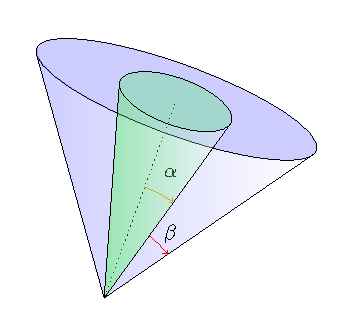
\includegraphics[scale=0.7]{cone.pdf}
\end{column}
\end{columns} 
 
\end{frame}

\begin{frame}{(1) TauFinder Optimization}
\begin{columns}
\begin{column}{0.5\textwidth}
Optimization of 3 parameters:\\
\scriptsize
-- SearchCone $\alpha$  $\in \, [0,0.15] $ rad with $0.01 $ rad steps\\
-- IsolationCone $\beta$ $\in \, [0,0.15] $ rad with $0.01 $ rad steps\\
-- IsolationEnergy $E_{iso}$ $\in \, [0,5.5] $ GeV with $0.5 $ GeV steps \\

For simplicity, fix invariant mass cut $\leq$ 2 GeV
\end{column}
\begin{column}{0.5\textwidth}
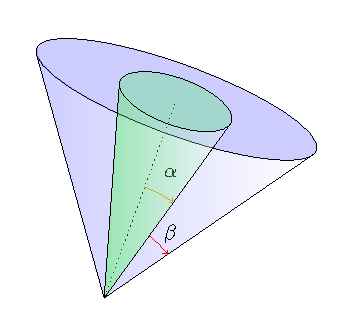
\includegraphics[scale=0.6]{cone.pdf}
\end{column}
\end{columns}

\textbf{Optimization metric} definitions:\\
\begin{columns}
\begin{column}{0.5\textwidth}
\textbf{Efficiency for true leptons} \\
\scriptsize using $WW\rightarrow qq \ell \nu$ 
\\
\colorbox{yellow}{$\varepsilon_s = N_{matched}/N_{Stotal} $}\\
	\scriptsize
	\begin{itemize}
	\item[-] $N_{matched} \geq$ 1 candidate matched within 100 mrads of the Gen. lepton/visible components\\ 
	\item[-] $N_{Stotal}$ includes an acceptance cut with 3 visible Gen. fermions $|cos\theta |< 0.99$
	\end{itemize}
	\normalsize	
	Optimal working point at:\\
	\quad \quad \quad \colorbox{green}{ max$[(1-P_{fake}) \varepsilon_s]$}
\end{column}
\begin{column}{0.5\textwidth}
\textbf{Probability of fake leptons}\\
\scriptsize using $WW \rightarrow qqqq$ \\
\colorbox{yellow}{$P_{fake} = 1-(1 - \varepsilon_b)^{\frac{1}{4} }$}\\

\colorbox{yellow}{ $\varepsilon_b = N_b/N_{Btotal}$} \\
	\scriptsize
	\begin{itemize}
	\item[-] $P_{fake} =$ probability of 1 success(fake) given 1 trial(jet)\\
	\item[-] $N_b \geq$ 1 reconstructed lepton jet from all 4 jets\\
	\item[-] $N_{Btotal}$ includes an acceptance cut with 4 visible Gen. fermions $|cos\theta |< 0.99$
	\end{itemize}

\end{column}
\end{columns}

\end{frame}

\begin{frame}{(1) TauFinder Optimization Results}
\scriptsize
Optimized against $qq\ell \nu$ and $qqqq$ samples with $100\% \, \, e^-_L e^+_R$ polarization 
\begin{tabular}{|p{0.15\textwidth}|p{0.1\textwidth}p{0.1\textwidth}p{0.1\textwidth}p{0.1\textwidth}p{0.1\textwidth}p{0.1\textwidth}|}

\hline 
\rowcolor{lightgray}
Channel & $\varepsilon_s$ & $1-P_{fake}$ & \% Matched & searchCone [rad] & isoCone [rad] & isoE [GeV] \\ 
\hline 
\rowcolor{green}
Prompt $\mu$ & 0.905 & 0.974 & 0.992 & 0.03 & 0.15 & 3.0 \\ 
\rowcolor{emerald}
Inclusive $\tau$ & 0.736 & 0.943 & 0.958 & 0.07 & 0.15 & 4.5 \\ 
 
$\tau \rightarrow \nu \nu \mu$ & 0.802 & 0.974 & 0.984 & 0.03 & 0.15 & 3.0 \\ 
 
$\tau \rightarrow \nu \nu e$ & 0.781 & 0.963 & 0.981 & 0.05 & 0.15 & 3.5 \\ 
 
$\tau$ Had-1p & 0.707 & 0.943 & 0.951 & 0.07 & 0.15 & 4.5 \\ 
 
$\tau$ Had-3p & 0.709 & 0.930 & 0.937 & 0.07 & 0.15 & 5.5 \\ 
 
Prompt $e$ & 0.839 & 0.961 & 0.970 & 0.04 & 0.15 & 4.0 \\ 
\hline 
\end{tabular} 
\quad \quad \\
\quad \quad \\
\begin{itemize}
\item Trickier reconstruction suggests wider cones and more isolation energy
\item Use two cones for analysis \colorbox{green}{Prompt $\mu$} and \colorbox{emerald}{Inclusive $\tau$} for a \colorbox{green}{Tight} and \colorbox{emerald}{Loose} selection
\item Expect tight selection to best capture all high quality lepton candidates
\item Loose selection should boost efficiency of hadronic $\tau$
\end{itemize}




\end{frame}

\begin{frame}{(2) Hadronic System}

\begin{columns}
\begin{column}{0.5\textwidth}
If a lepton has been found, 
\begin{itemize}
\scriptsize
\item[-]select highest energy candidate as signal lepton\\
\item[-] shuffle remaining fakes back into the hadronic system.\\
\end{itemize}
\scriptsize
At least one quark tends to be very forward, so pileup tends to mix into the jets\\
\quad \quad \\
These beam particles cannot be cleanly removed by standard methods e.g. kT algorithm with tuned R values\\

\end{column}
\begin{column}{0.5\textwidth}

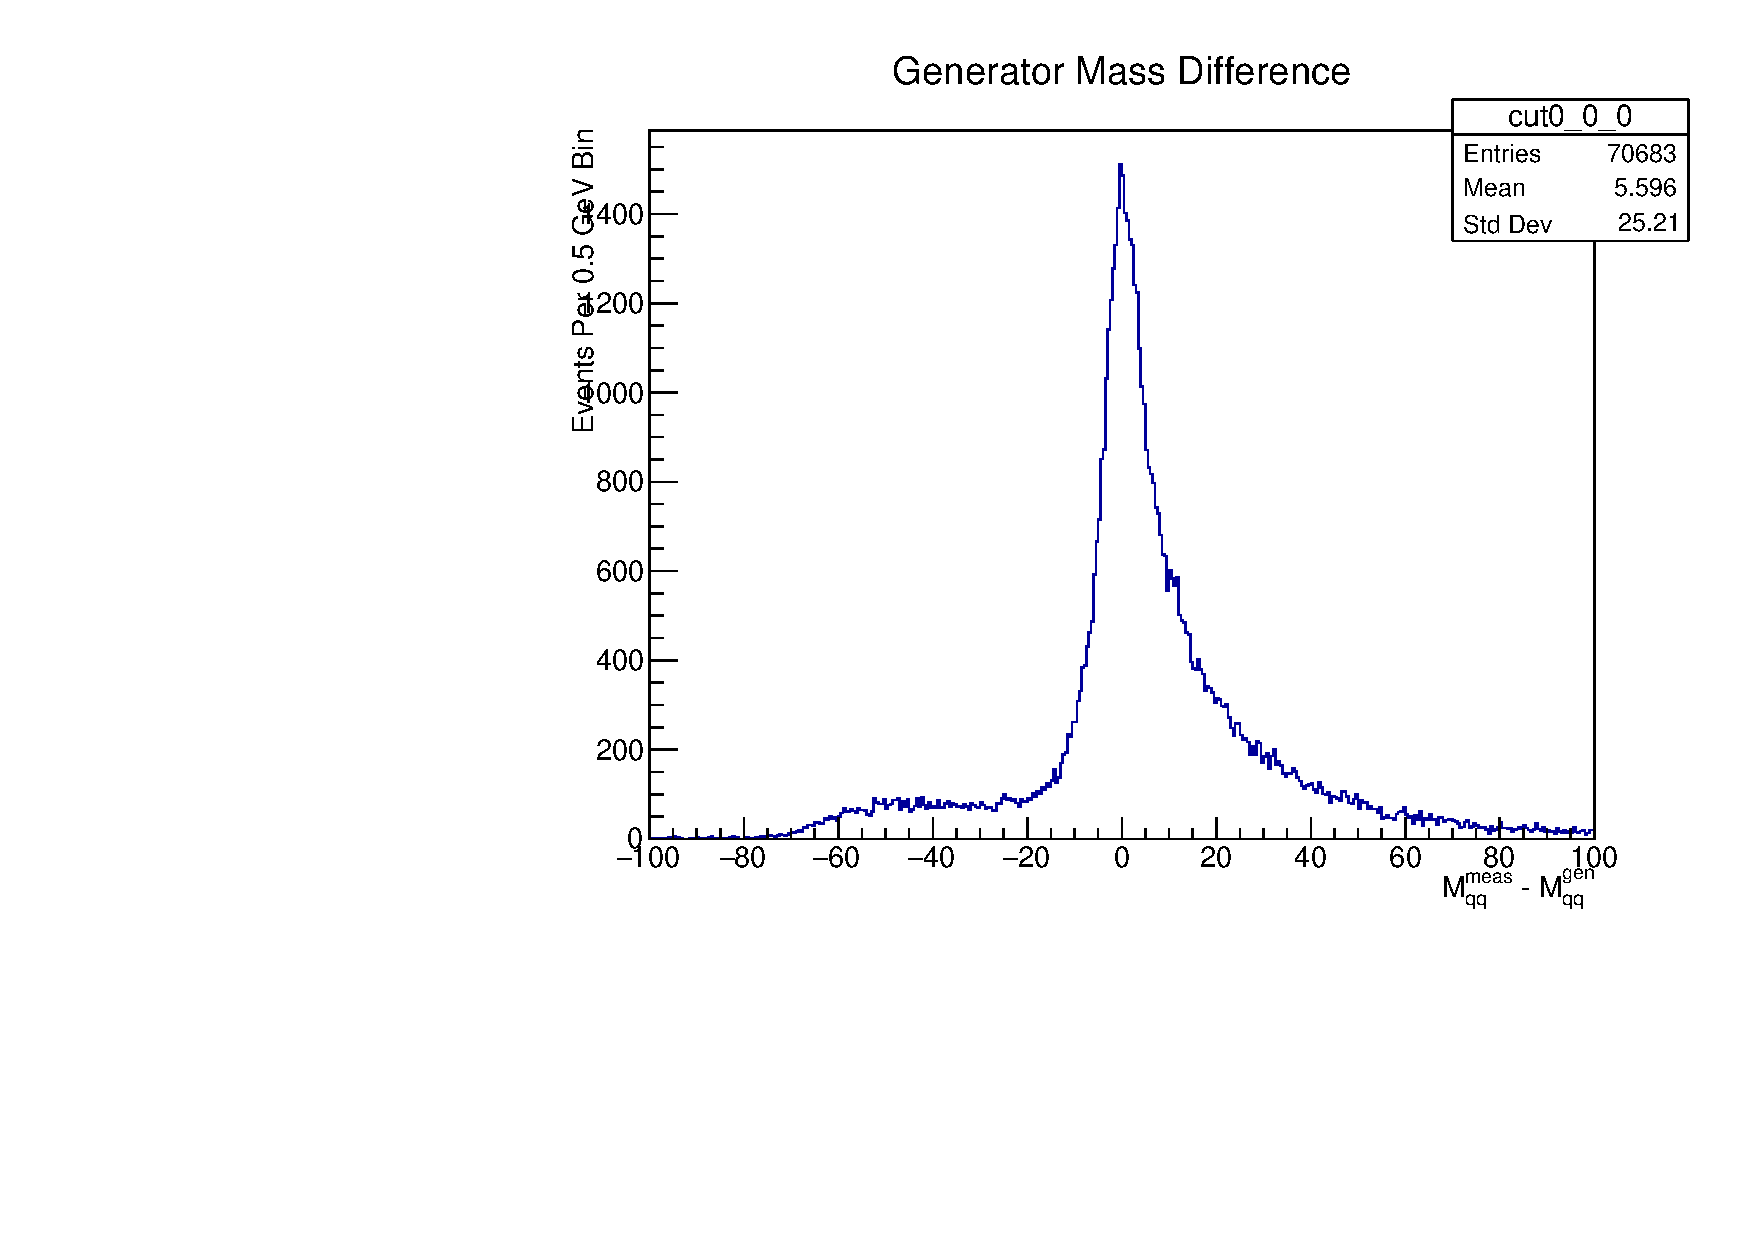
\includegraphics[scale=0.3]{nocutDiff.pdf}\\
\scriptsize
\quad $100\% \, \, e^-_L e^+_R$ polarization\\
 Measured mass is often larger than the true value \\



\end{column}
\end{columns}
\normalsize
Mitigate Pileup with ``Jet Fragmentation"\\
  \begin{itemize}
  	\scriptsize
  \item[-]tune y-cut($\propto M^2_{jet}$) values on the durham algorthim (eekt)
  \item[-]apply simple cuts to the resulting ``mini-jets"\\
  \end{itemize}

\end{frame}
\begin{frame}{(2) Optimized W Mass}
Find best W jet parameters with signal prompt muons\\
\scriptsize
Jet Clustering -- yCut:$[1\times10^{-3}, 5\times10^{-6}]$ \\

$\text{Kinematic cuts} - 
\begin{cases}
	pT:[0,5]\, \, \text{bins of} \, \, 0.5 \text{GeV} \\
	|cos\theta|:[0.9,1] \, \, 0.01 \text{bins}
	\end{cases}
$\\
\quad \quad \\
\normalsize
\quad \quad \\
Use 2 optimization parameters from the $M_{qq}^{meas} - M_{qq}^{gen}$ dist.:\\
\begin{itemize}
\item[-] Full Width Half Maximum (FWHM) \\
\item[-]Number of bin Entries in the Mode\\
\end{itemize}
\quad \quad \\ 
\scriptsize
The Mode Entries is the number of entries in the Maximum bin + the number of Entries of the nearest left/right neighbor bins\\
The Mode is the weighted mean of the center of the 3 Mode bins\\
\quad \quad \\ 
The Maximum for the FWHM is the "Mode Average" or the average number of entries from the 3 mode bins\\
\quad \quad \\ 
The edges of the Width for FWHM are the weighted average between the 2 bins around the half maximum ( 1 bin above 1 bin below) 
\end{frame}

\begin{frame}{(2) Hadronic System Results}

\begin{columns}
\begin{column}{0.5\textwidth}
   	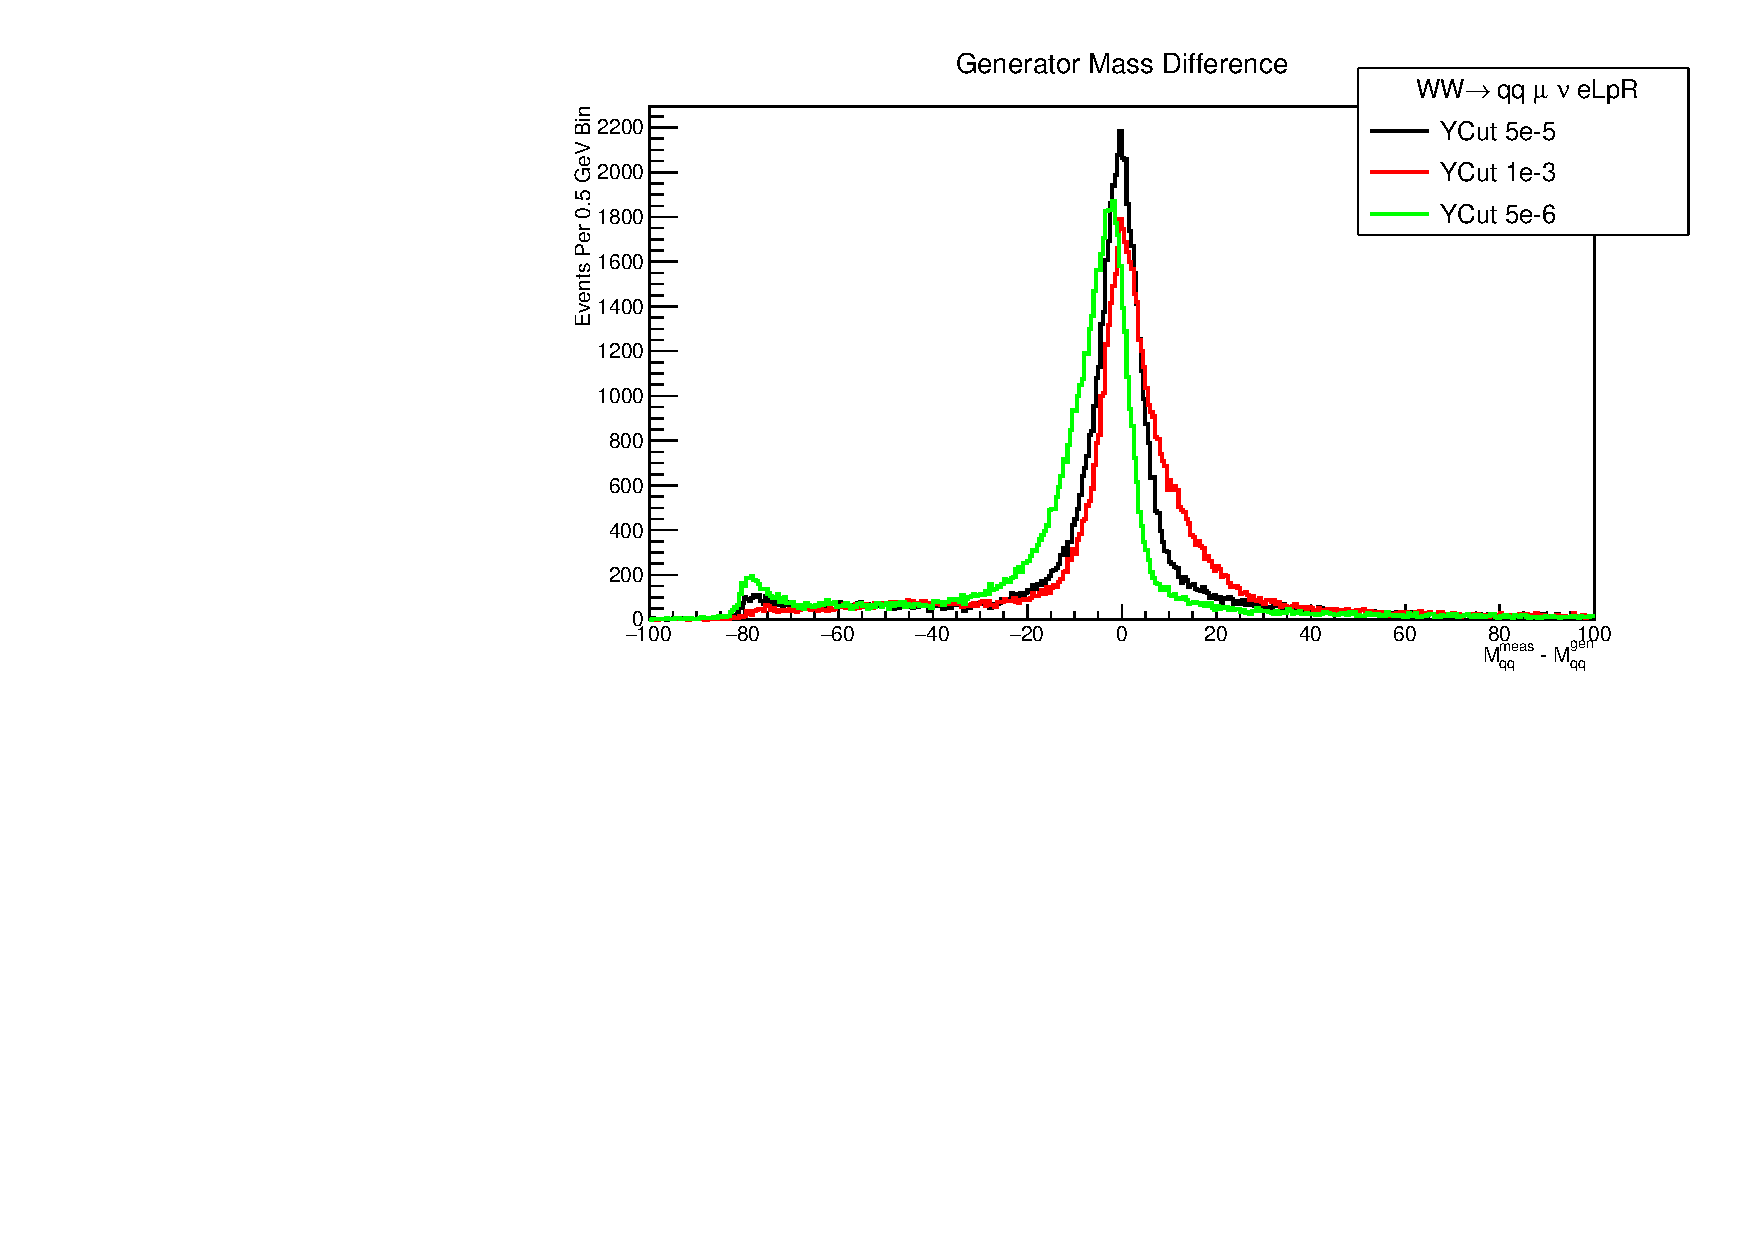
\includegraphics[scale=0.3, left]{SupDiff.pdf}\\
   	\scriptsize
   	Comparison of 3 YCuts with the same kinematic cuts Pt$>$2 GeV AND $|cos\theta|<$1 (optimized for 5e-05)\\
   	\quad \quad \\
   	Small peak around -80 GeV is where the W has been incorrectly thrown out\\
   	\quad \quad \\
   	
   
\end{column}
\begin{column}{0.5\textwidth}
	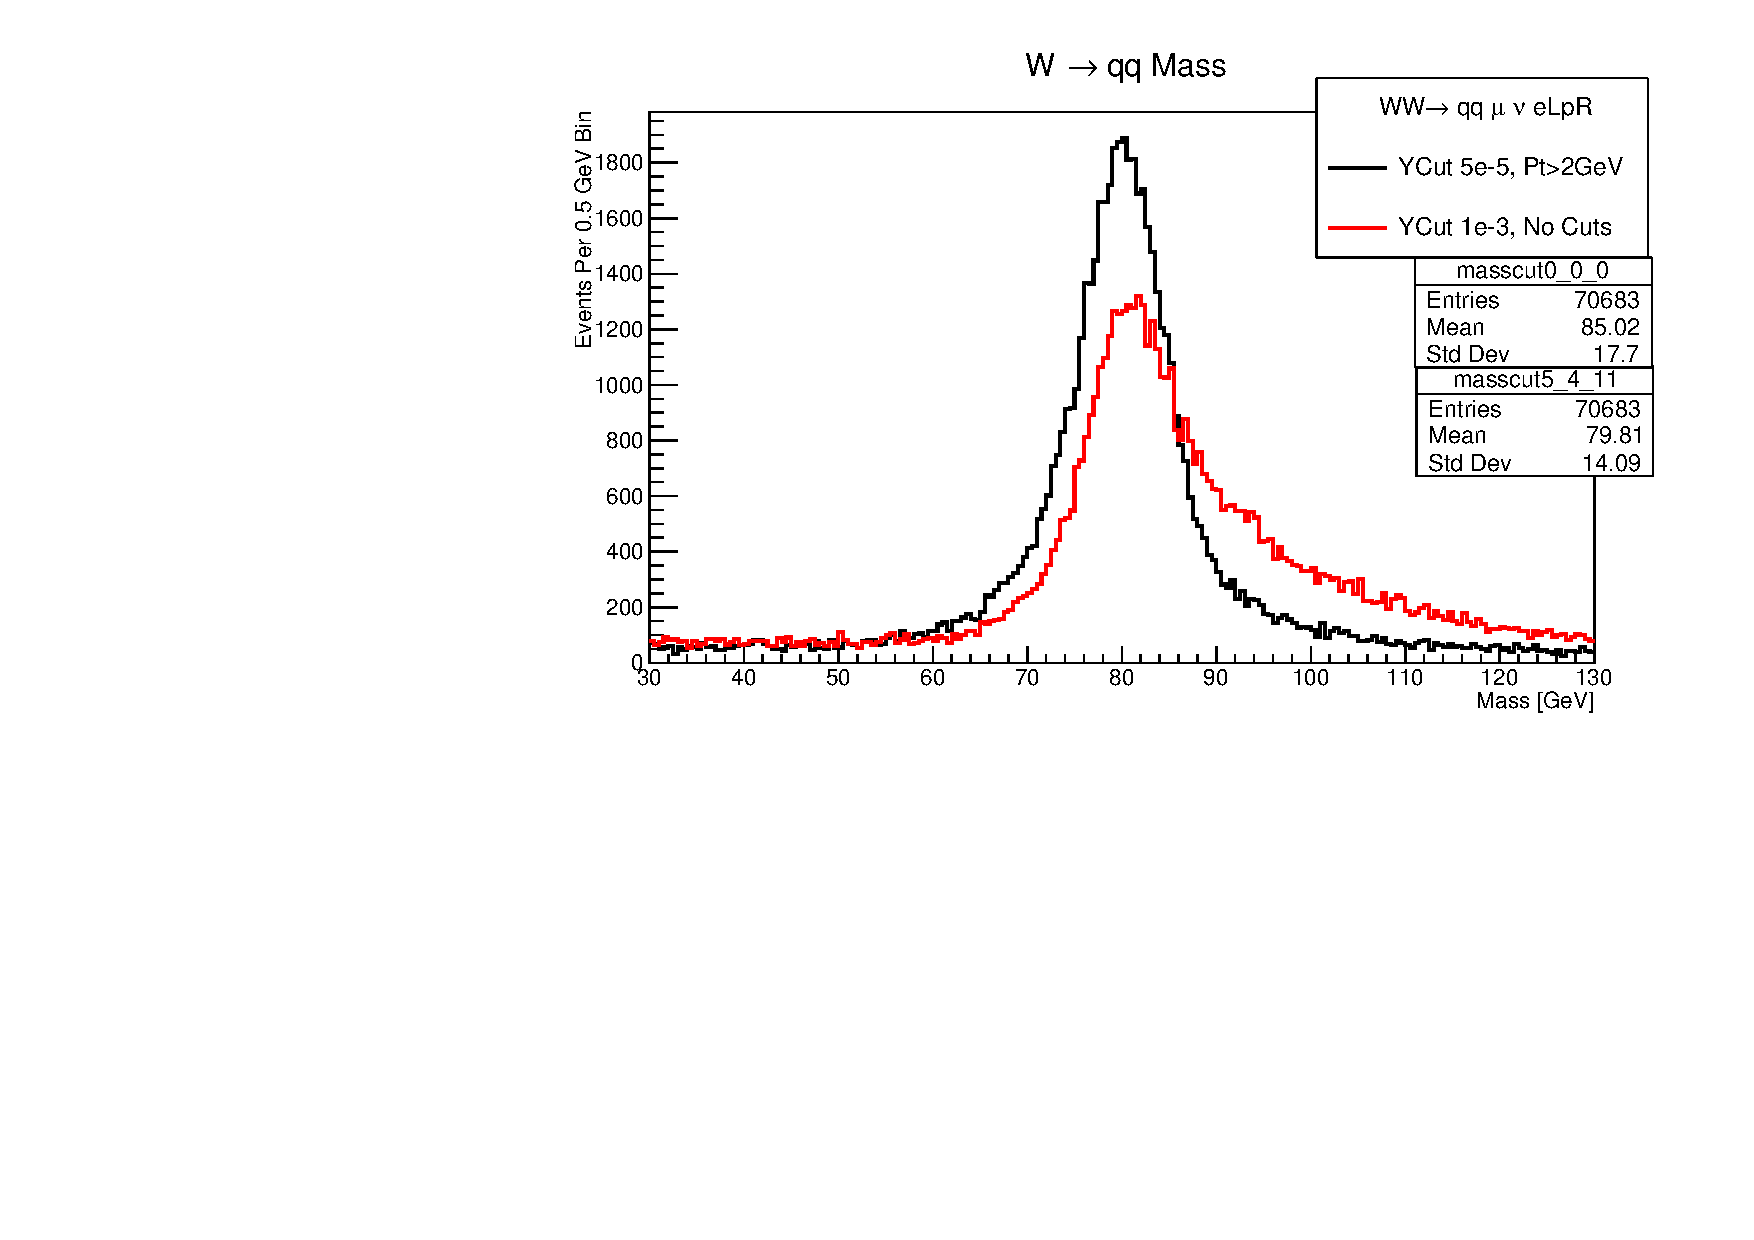
\includegraphics[scale=0.3, left]{SupMass.pdf}\\
	\scriptsize
	\quad \quad \quad \quad Significant Improvement !
\end{column}	
\end{columns}
\tiny
 Mass Difference Statistics:\\
 ycut: 0.001  ptcut: 2  costcut: 1  FWHM: 11.769 RMS: 24.1855 Mode: -0.24211 mean: 0.782898 modeEnt: 5199\\
 ycut: 5e-05  ptcut: 2  costcut: 1  FWHM: 9.7087 RMS: 25.2774 Mode: -0.25127 mean: -3.09776 modeEnt: 6326\\
 ycut: 5e-06  ptcut: 2  costcut: 1  FWHM: 11.567 RMS: 25.7475 Mode: -1.75521 mean: -9.57673 modeEnt: 5475\\

\quad \quad \\
\normalsize
Best Performance is reached with:\\
\textbf{ycut= 5e-05 and removal of mini-jets with pT $<$ 2 GeV }


\end{frame}
\begin{frame}{(3) Event Selection Overview}
Perform event selection with two mutually exclusive groups:\\
1st group will use $\mu$ cone (optimized for prompt muons)
	\begin{itemize}
		\scriptsize
		\item[-]\colorbox{green}{Tight} selection will yield some \colorbox{green}{efficiency $\epsilon_0$ and purity $p_0$}
		\item[-] tight cuts will be targeted towards prompt signal leptons $\mu/e$ 
	\end{itemize} 
2nd group will use the $\tau$ cone (optimized for inclusive $\tau$ decays)
	\begin{itemize}
	\scriptsize
		\item[-] \colorbox{emerald}{Loose} selection will yield some \colorbox{emerald}{efficiency $\epsilon_1$ and purity $p_1$}
		\item[-] Loose cuts should address $\tau$s not reconstructed by muon cone
		\item[-] orthogonalize selection require 0 tight leptons in loose selection
	\end{itemize}
Overall efficiency \colorbox{yellow}{$\epsilon = \epsilon_0 + \epsilon_1$}\\
Overall purity \colorbox{yellow}{$p = (N_0 + N_1) / (B_0 + B_1 + N_0 +N_1)$}\\
\quad \quad \\


\end{frame}
\begin{frame}
Description of current cuts:(currently tight/loose are mostly the same)\\
\tiny
adapted from ref. \url{I. Marchesini DESY-THESIS 2011}\\
\scriptsize
--Note reconstucted particles are boosted against crossing angle boost-- (3.5 GeV in x)\\
\begin{itemize}
\item[-]\colorbox{orange}{Lepton} - Require at least 1 reconstructed lepton
\item[-]\colorbox{orange}{Track Multiplicity $> 10$} - more than 10 tracks in the event (Before pileup removal)
\item[-]\colorbox{orange}{Pt $> 5$ GeV} - Reject events with no genuine missing Pt 
\item[-]\colorbox{orange}{$E_{vis} < 500$ GeV} Sum of the total visible energy in the event 
\item[-]\colorbox{orange}{$E_{com} > 100$ GeV} - Rest-frame energy with visible and inferred missing energy\\  \quad $E_{com} = E_{vis} + |P_{miss}| \, \,  \, \text{and} \, \, P^\mu_{miss} = (|P_{miss}| , -\sum{\vec{p}_{vis}}) $
\item[-]\colorbox{orange}{$40<M_{qq}<120$} - constrains hadronic system to be W-like
\item[-]\colorbox{orange}{ $-qcos\theta_W$} - limit the $W^-$ backward scattering
\item[-]\colorbox{orange}{ $m^2_{\nu recoil} < 135,000 \, \, \text{GeV}^2$} - Require the visible system to recoil against a low mass object \\
\quad $m^2_{\nu recoil} = s + M^2_{vis} - 2\sqrt{s}E_{vis} \, \, \text{and} \, \, M^2_{vis} = ( P^{\mu}_{qq} +  P^{\mu}_{\ell})^2$ 

\end{itemize}
\end{frame}

\begin{frame}{(3) Event Selection (Tight)}
\scriptsize
Tight Signal $\Rightarrow$  muon cone for $\mu,e,\tau$ signal events\\
All plots include an N Lepton $> 0$ cut (except N Lepton plot)\\
Polarization: (-0.8,+0.3)\quad
Luminosity: 1600 fb$^{-1}$
\begin{columns}
\begin{column}{0.5\textwidth}
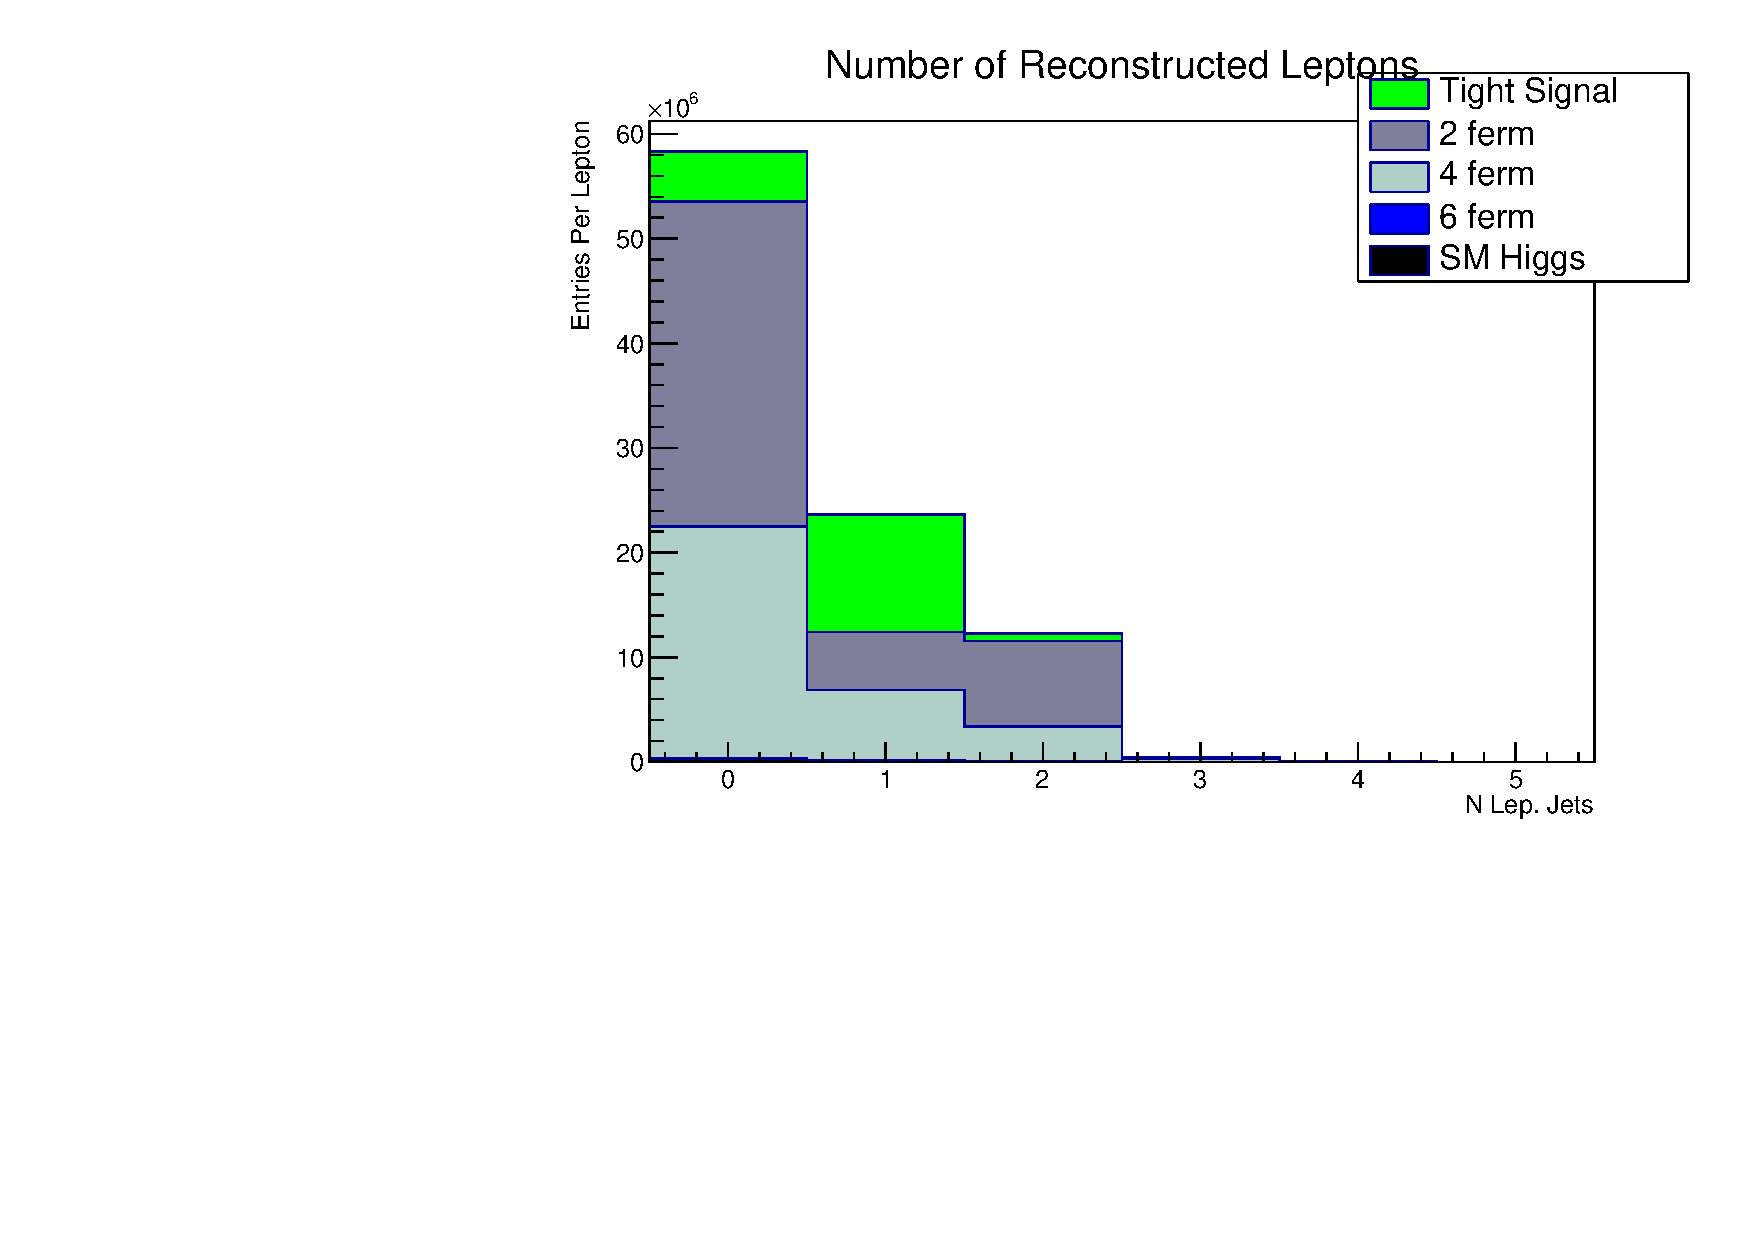
\includegraphics[scale=0.3, left]{nLepHist.pdf} \\
N Leptons $> 0$
\end{column}
\begin{column}{0.5\textwidth}
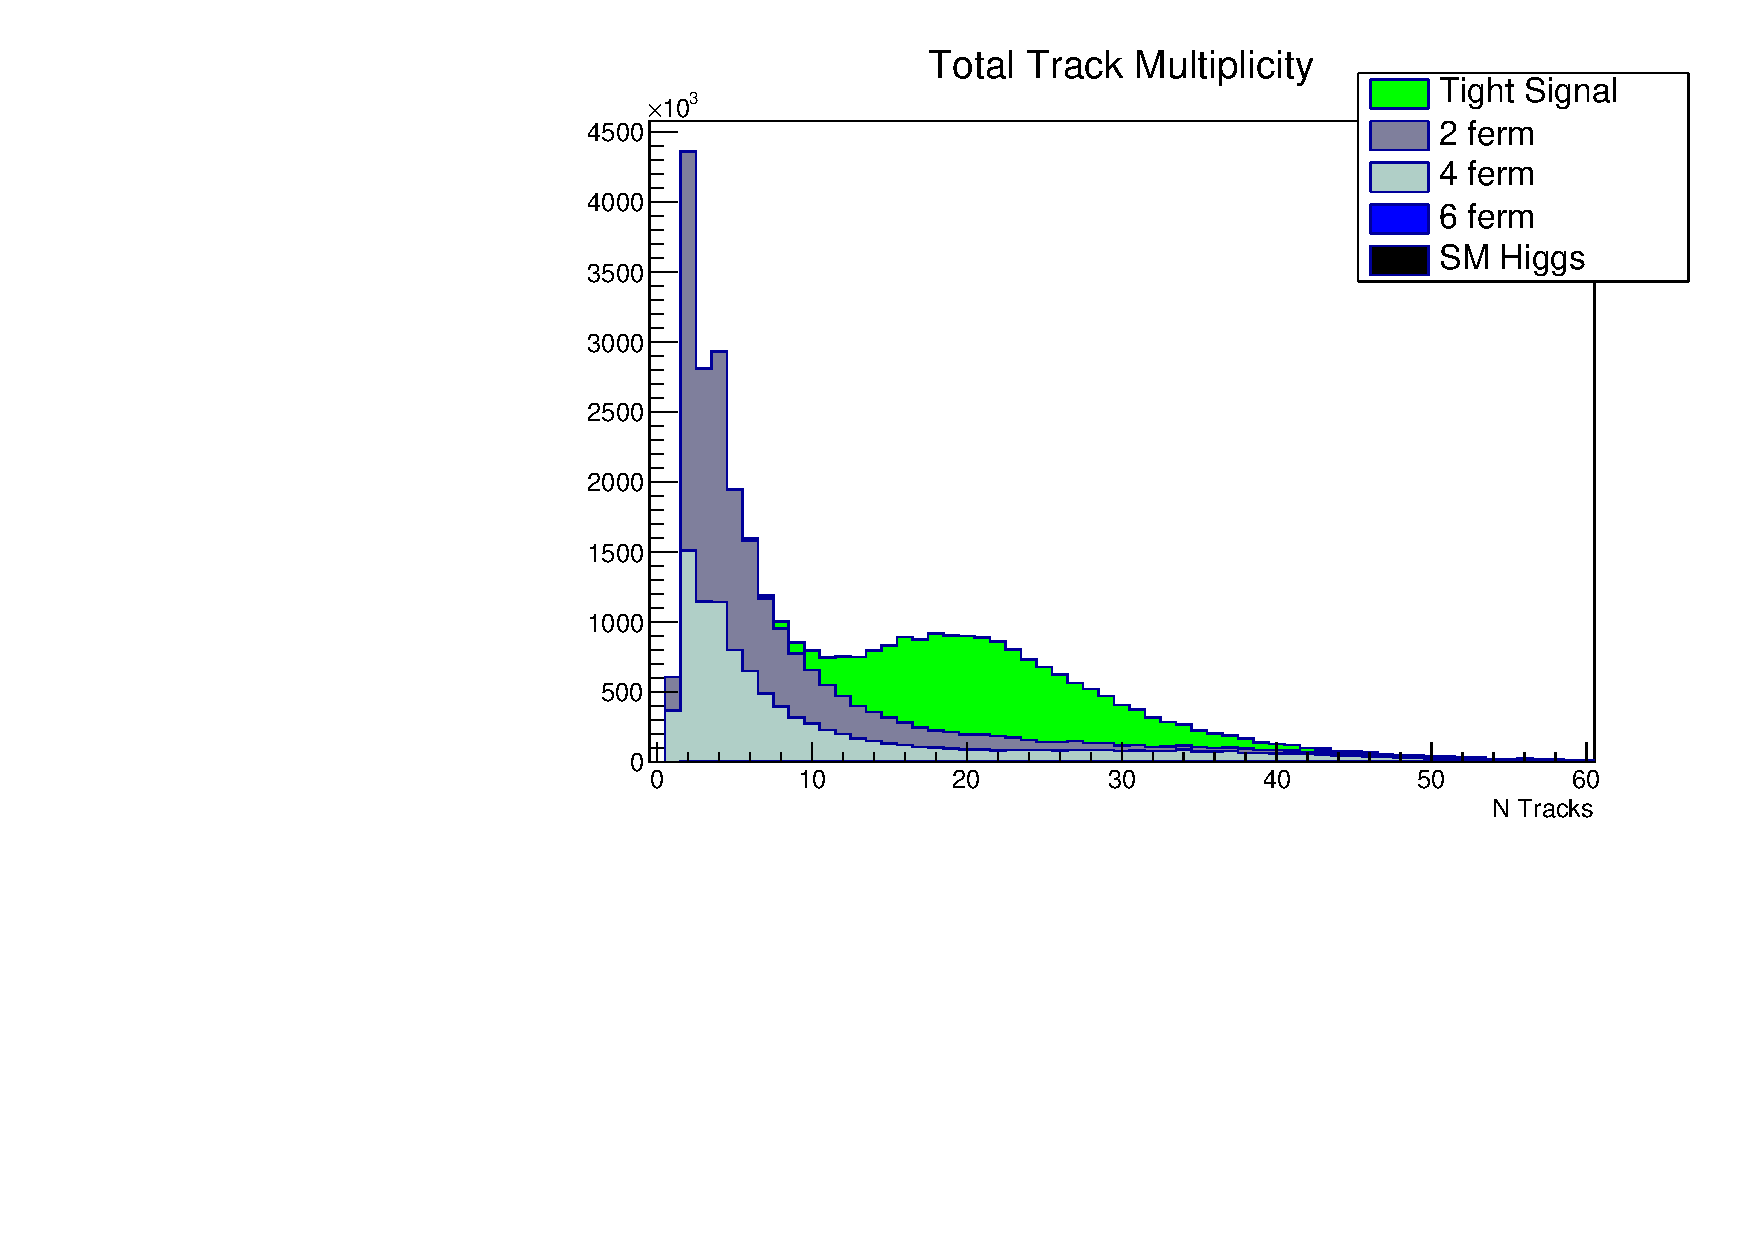
\includegraphics[scale=0.3, left]{ntracksHist.pdf} \\
N Tracks $> 10$
\end{column}
\end{columns}
\end{frame}

\begin{frame}{(3) Event Selection (Tight)}
\scriptsize
Tight Signal $\Rightarrow$  muon cone for $\mu,e,\tau$ signal events\\
All plots include an N Lepton $> 0$ cut\\
Polarization: (-0.8,+0.3)\quad
Luminosity: 1600 fb$^{-1}$
\begin{columns}
\begin{column}{0.5\textwidth}
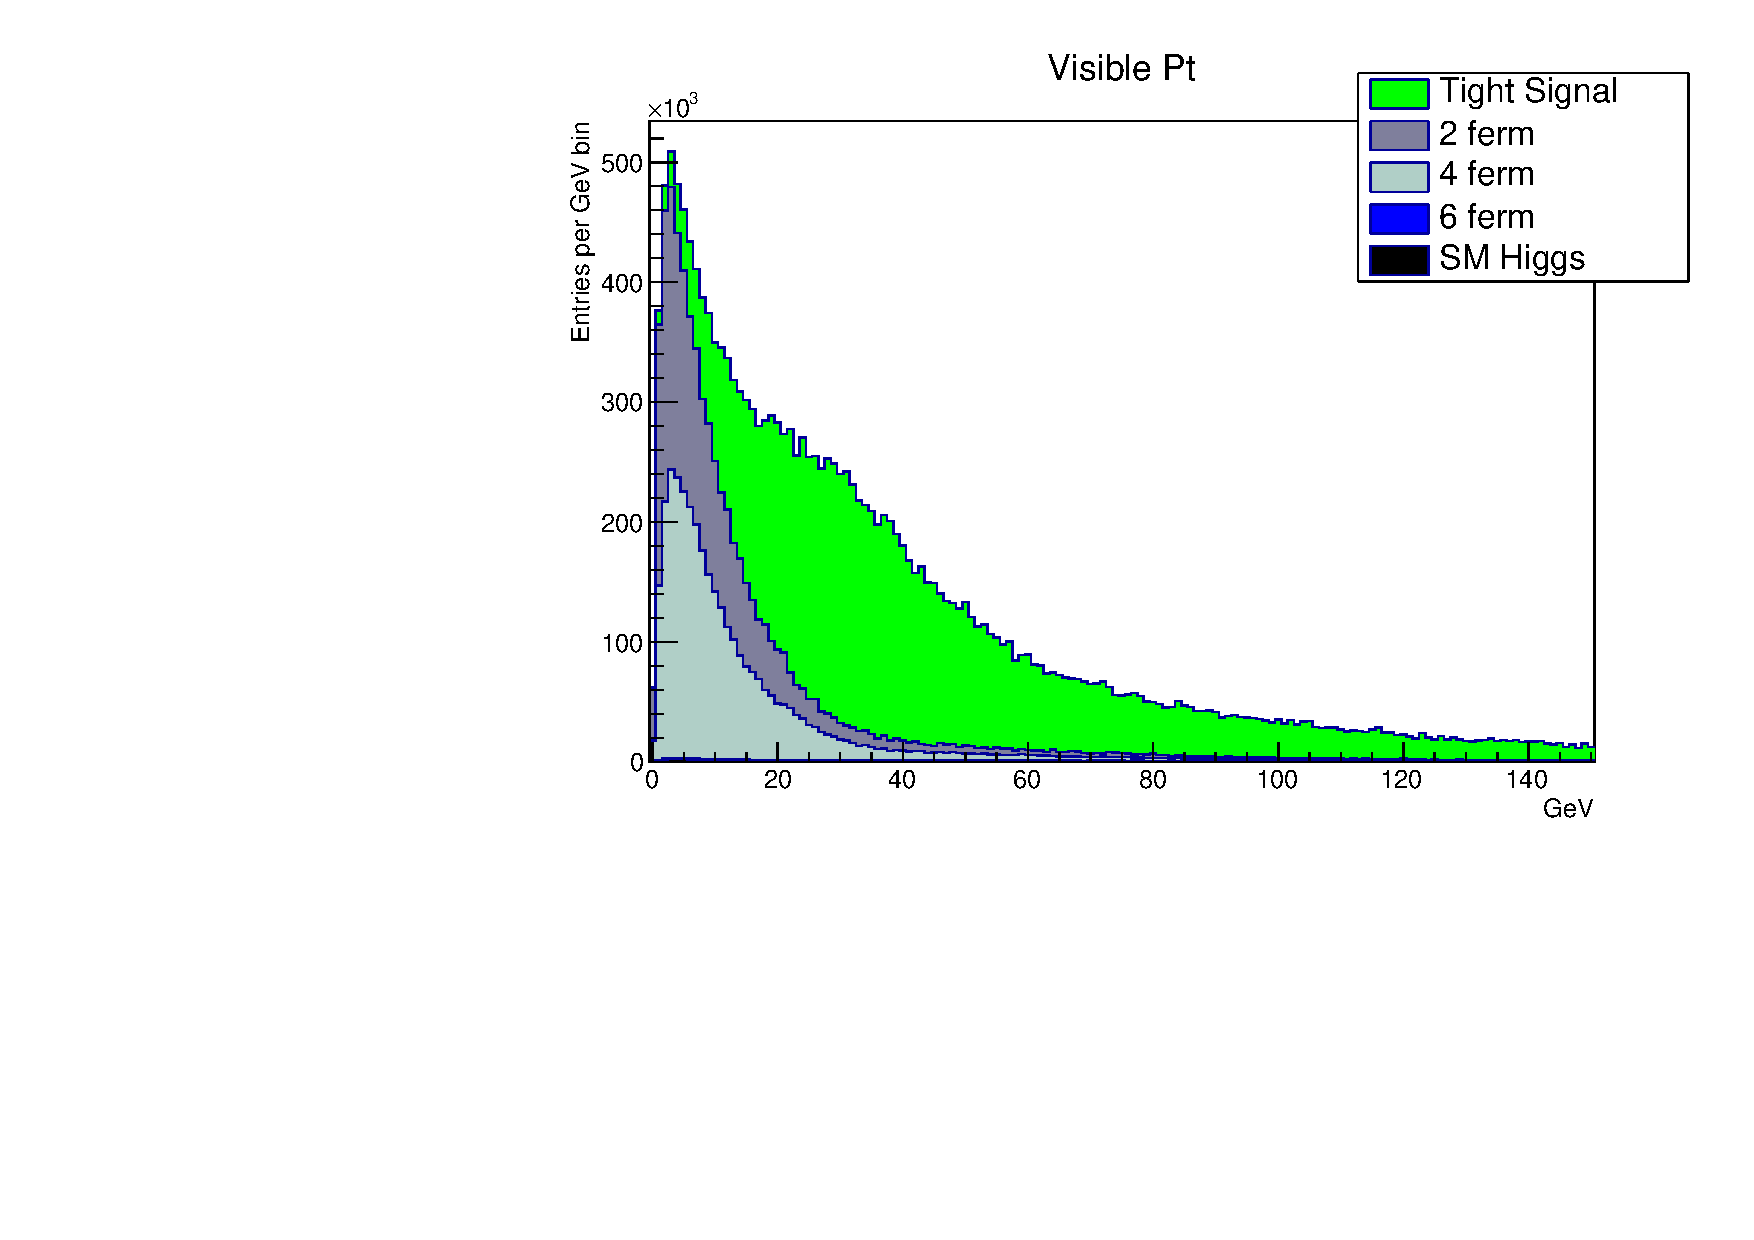
\includegraphics[scale=0.3, left]{PtvisHist.pdf} \\
Visible Pt $> 5$ GeV
\end{column}
\begin{column}{0.5\textwidth}
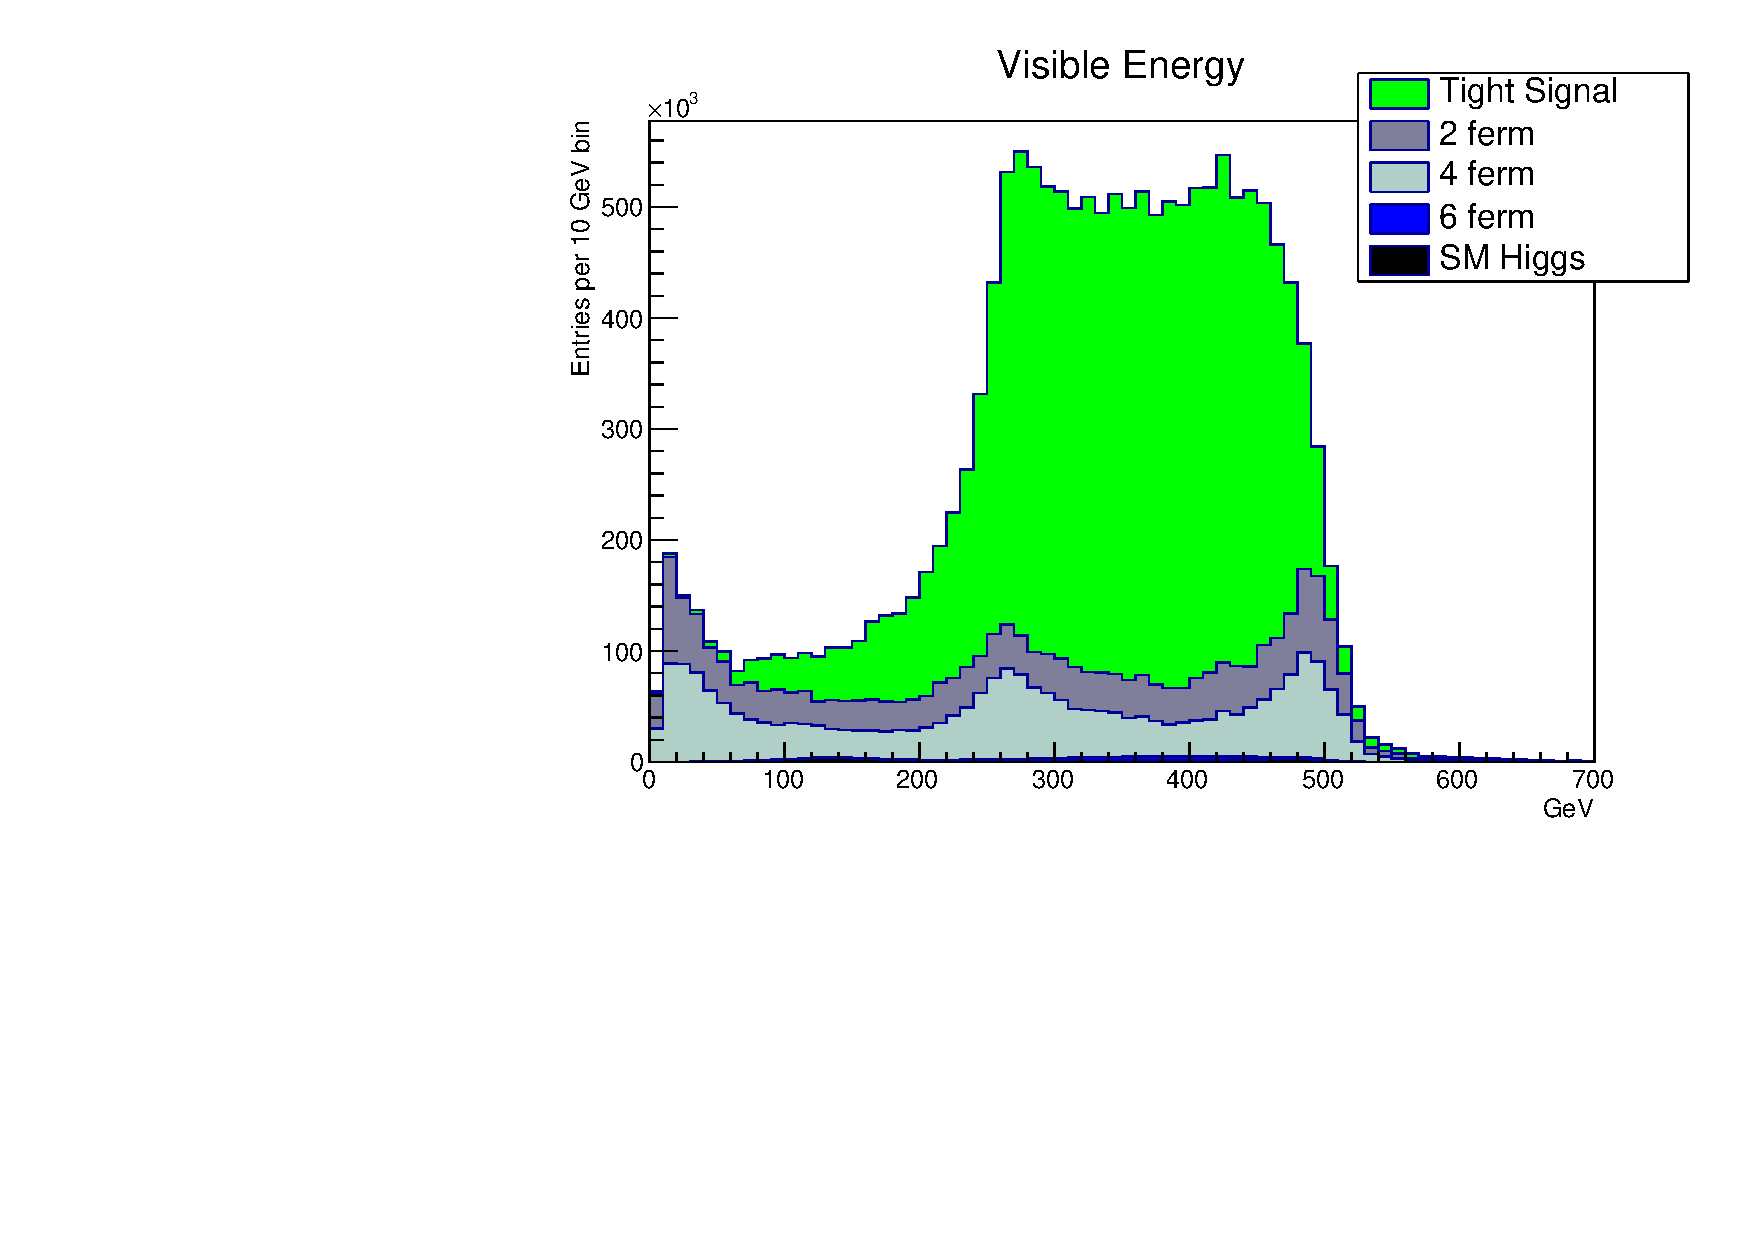
\includegraphics[scale=0.3, left]{EvisHist.pdf} \\
Visible Energy $< 500$ GeV
\end{column}
\end{columns}
\end{frame}

\begin{frame}{(3) Event Selection (Tight)}
\scriptsize
Tight Signal $\Rightarrow$  muon cone for $\mu,e,\tau$ signal events\\
All plots include an N Lepton $> 0$ cut\\
Polarization: (-0.8,+0.3)\quad
Luminosity: 1600 fb$^{-1}$
\begin{columns}
\begin{column}{0.5\textwidth}
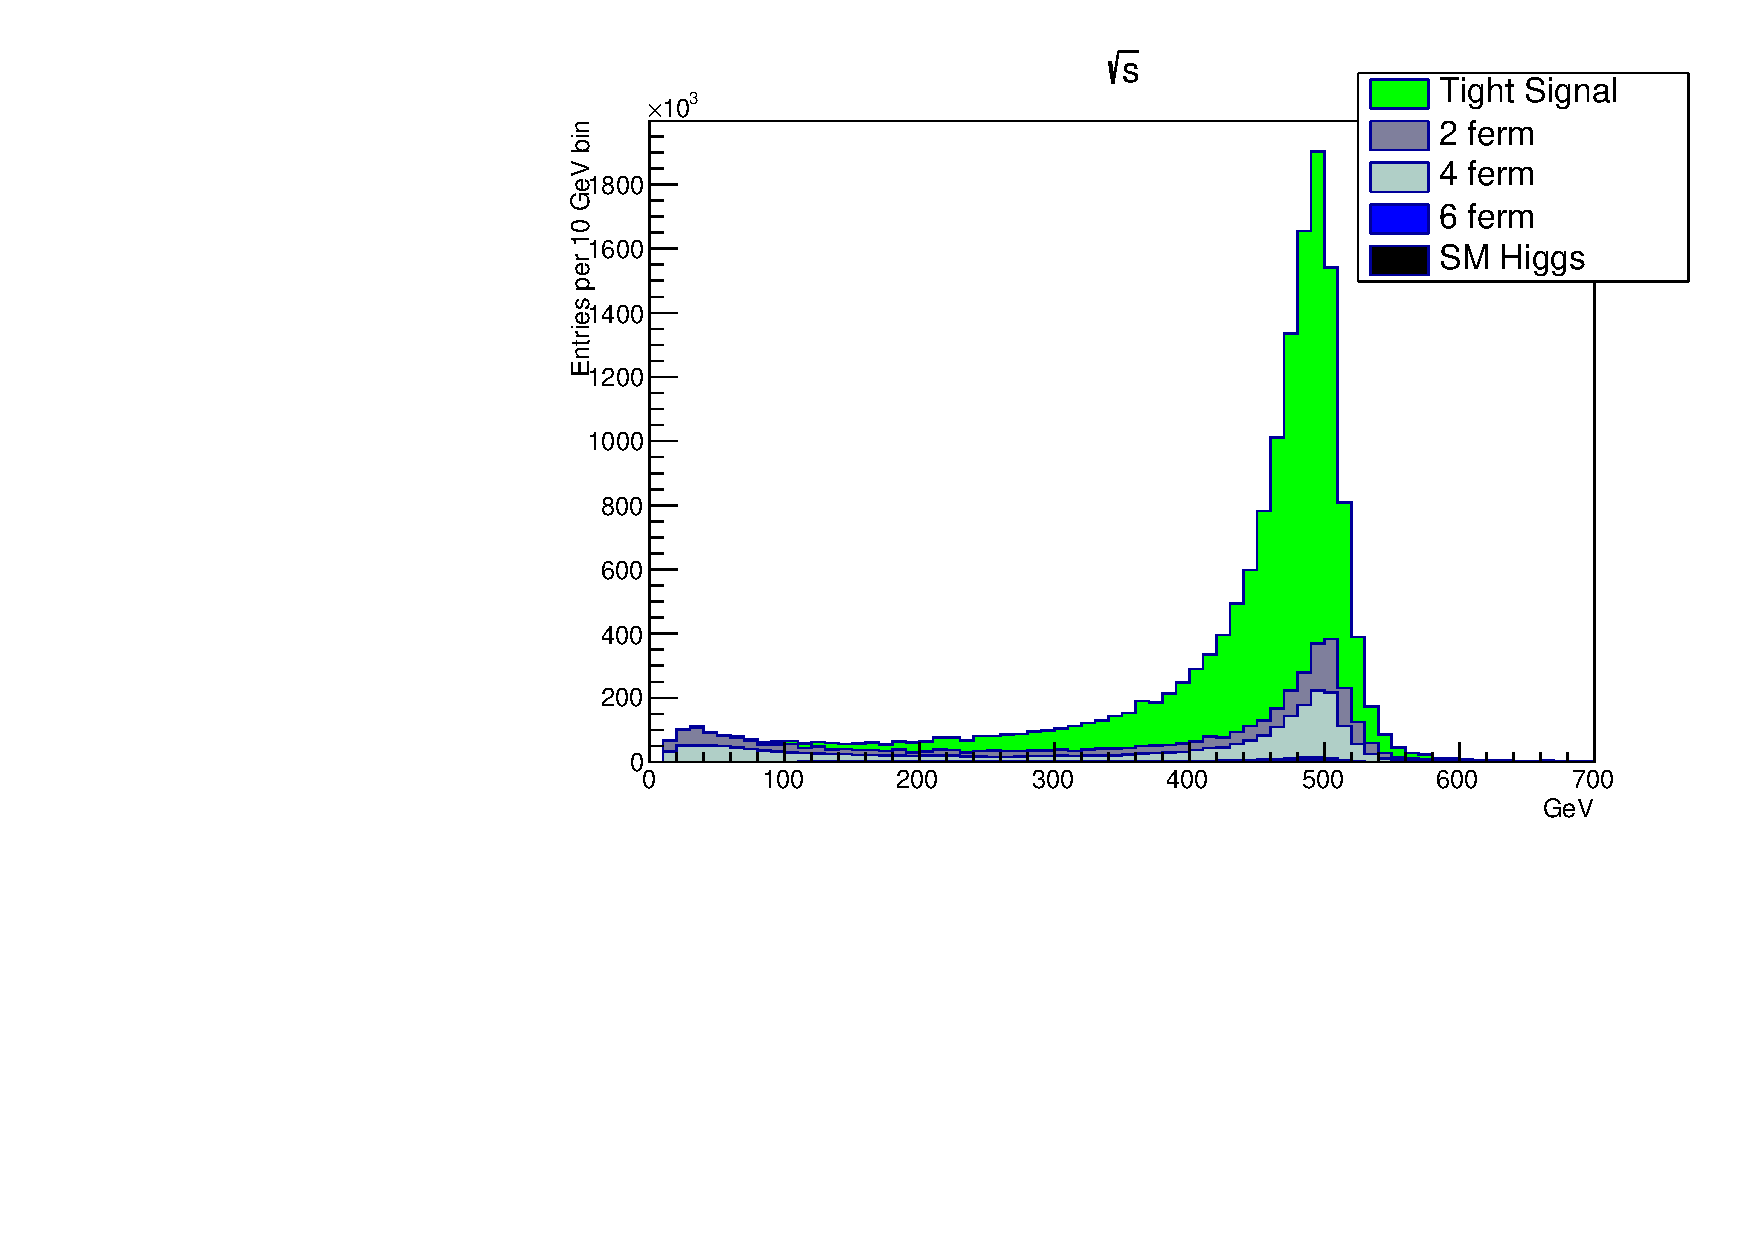
\includegraphics[scale=0.3, left]{EcomHist.pdf} \\
$E_{com} > 100$ GeV
\end{column}
\begin{column}{0.5\textwidth}
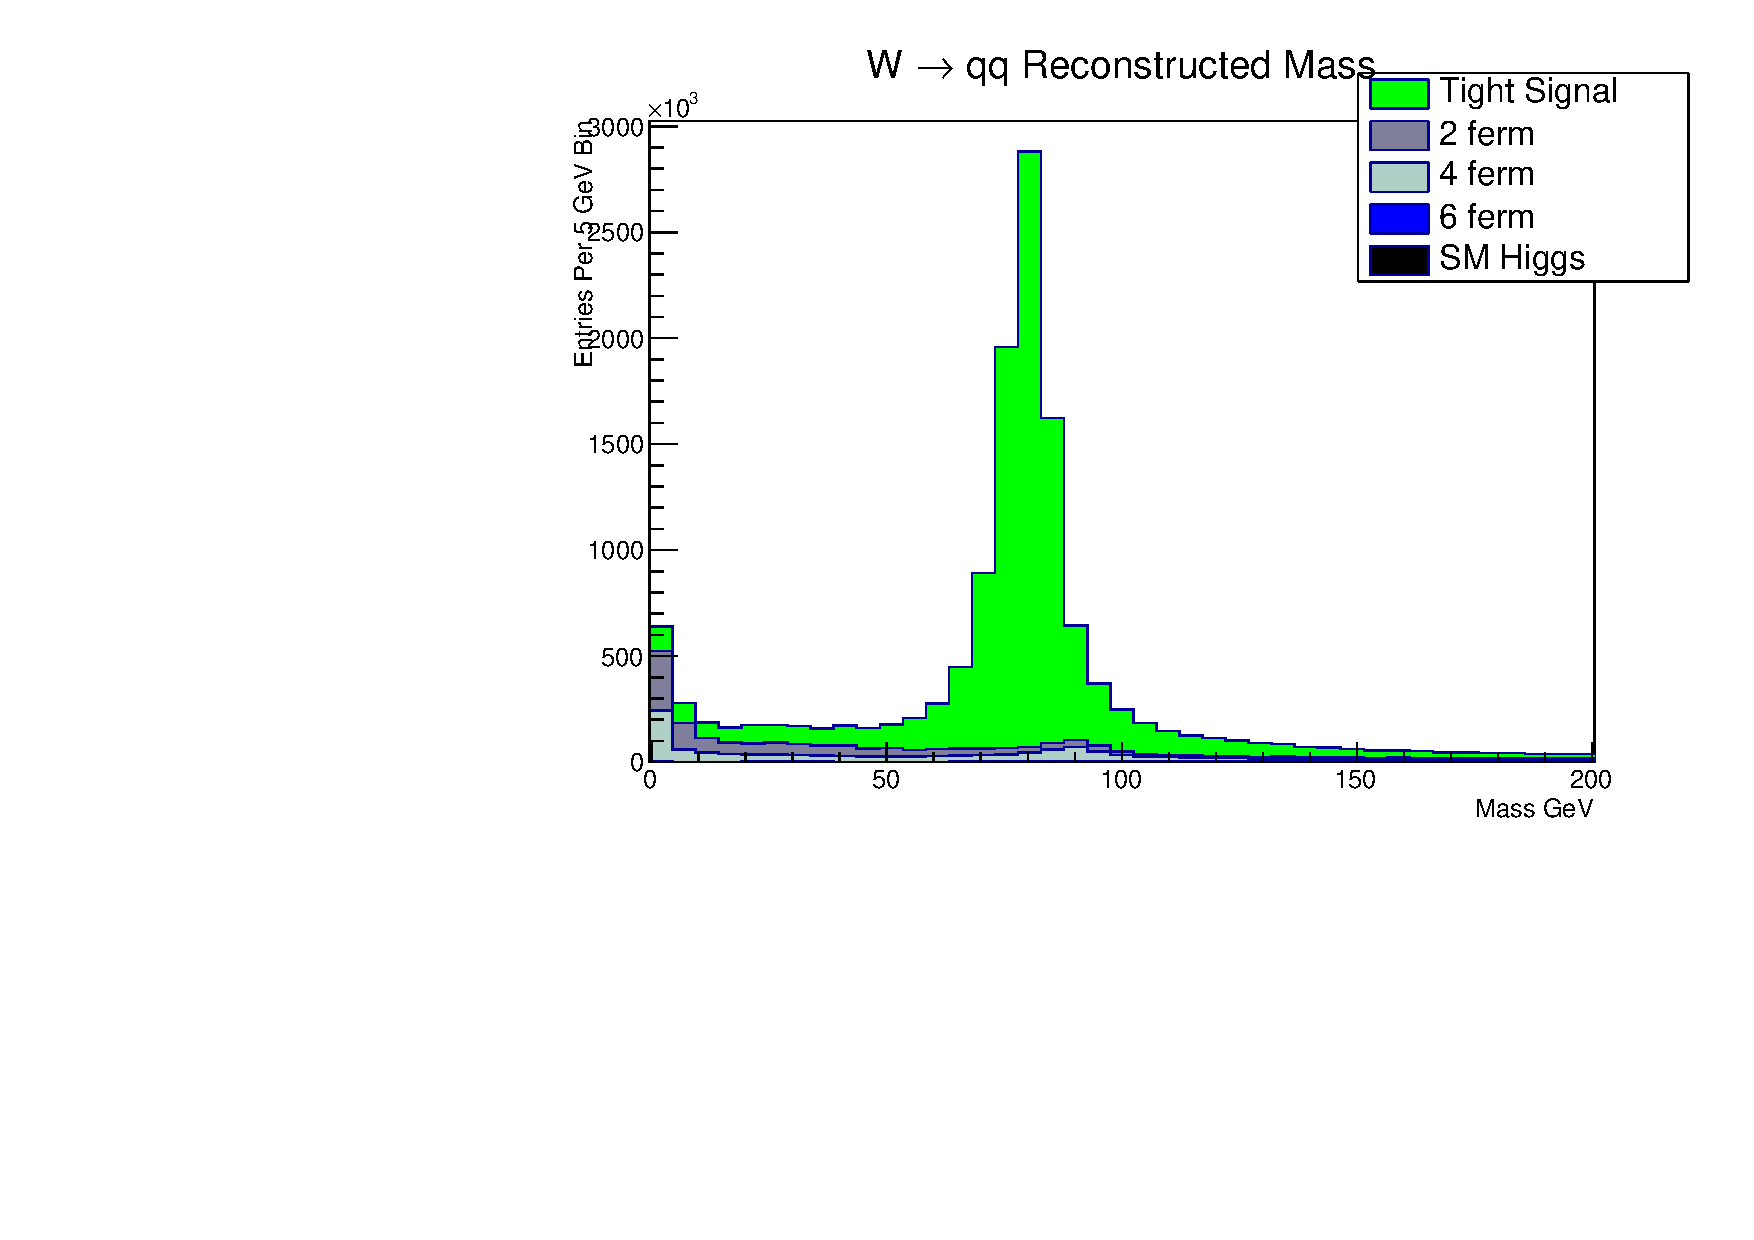
\includegraphics[scale=0.3, left]{mwhadHist.pdf} \\
$ 40 < M_{qq} < 120$
\end{column}
\end{columns}
\end{frame}

\begin{frame}{(3) Event Selection (Tight)}
\scriptsize
Tight Signal $\Rightarrow$  muon cone for $\mu,e,\tau$ signal events\\
All plots include an N Lepton $> 0$ cut\\
Polarization: (-0.8,+0.3)\quad
Luminosity: 1600 fb$^{-1}$\\
\begin{columns}
\begin{column}{0.5\textwidth}
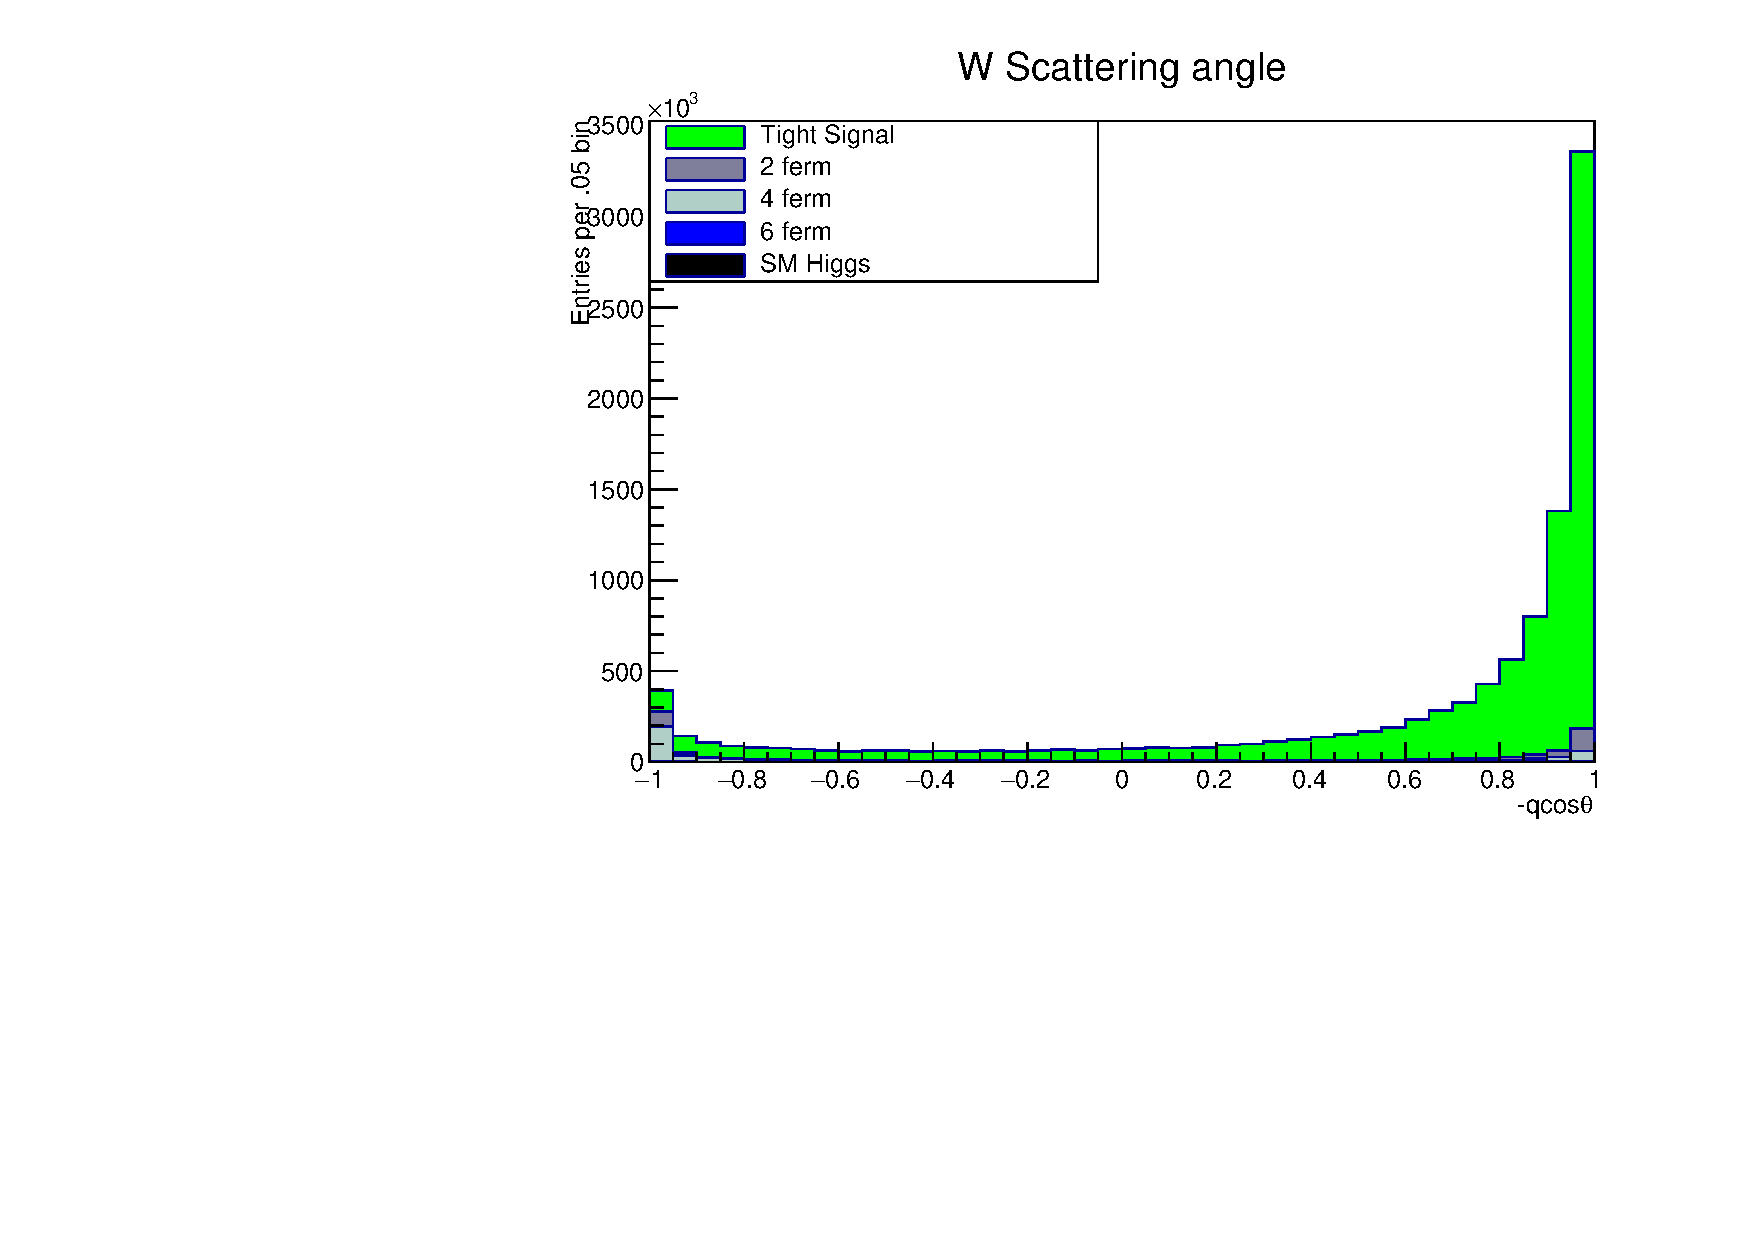
\includegraphics[scale=0.3, left]{qcostHist.pdf} \\
$-qcos\theta_W > -0.95$
\end{column}
\begin{column}{0.5\textwidth}
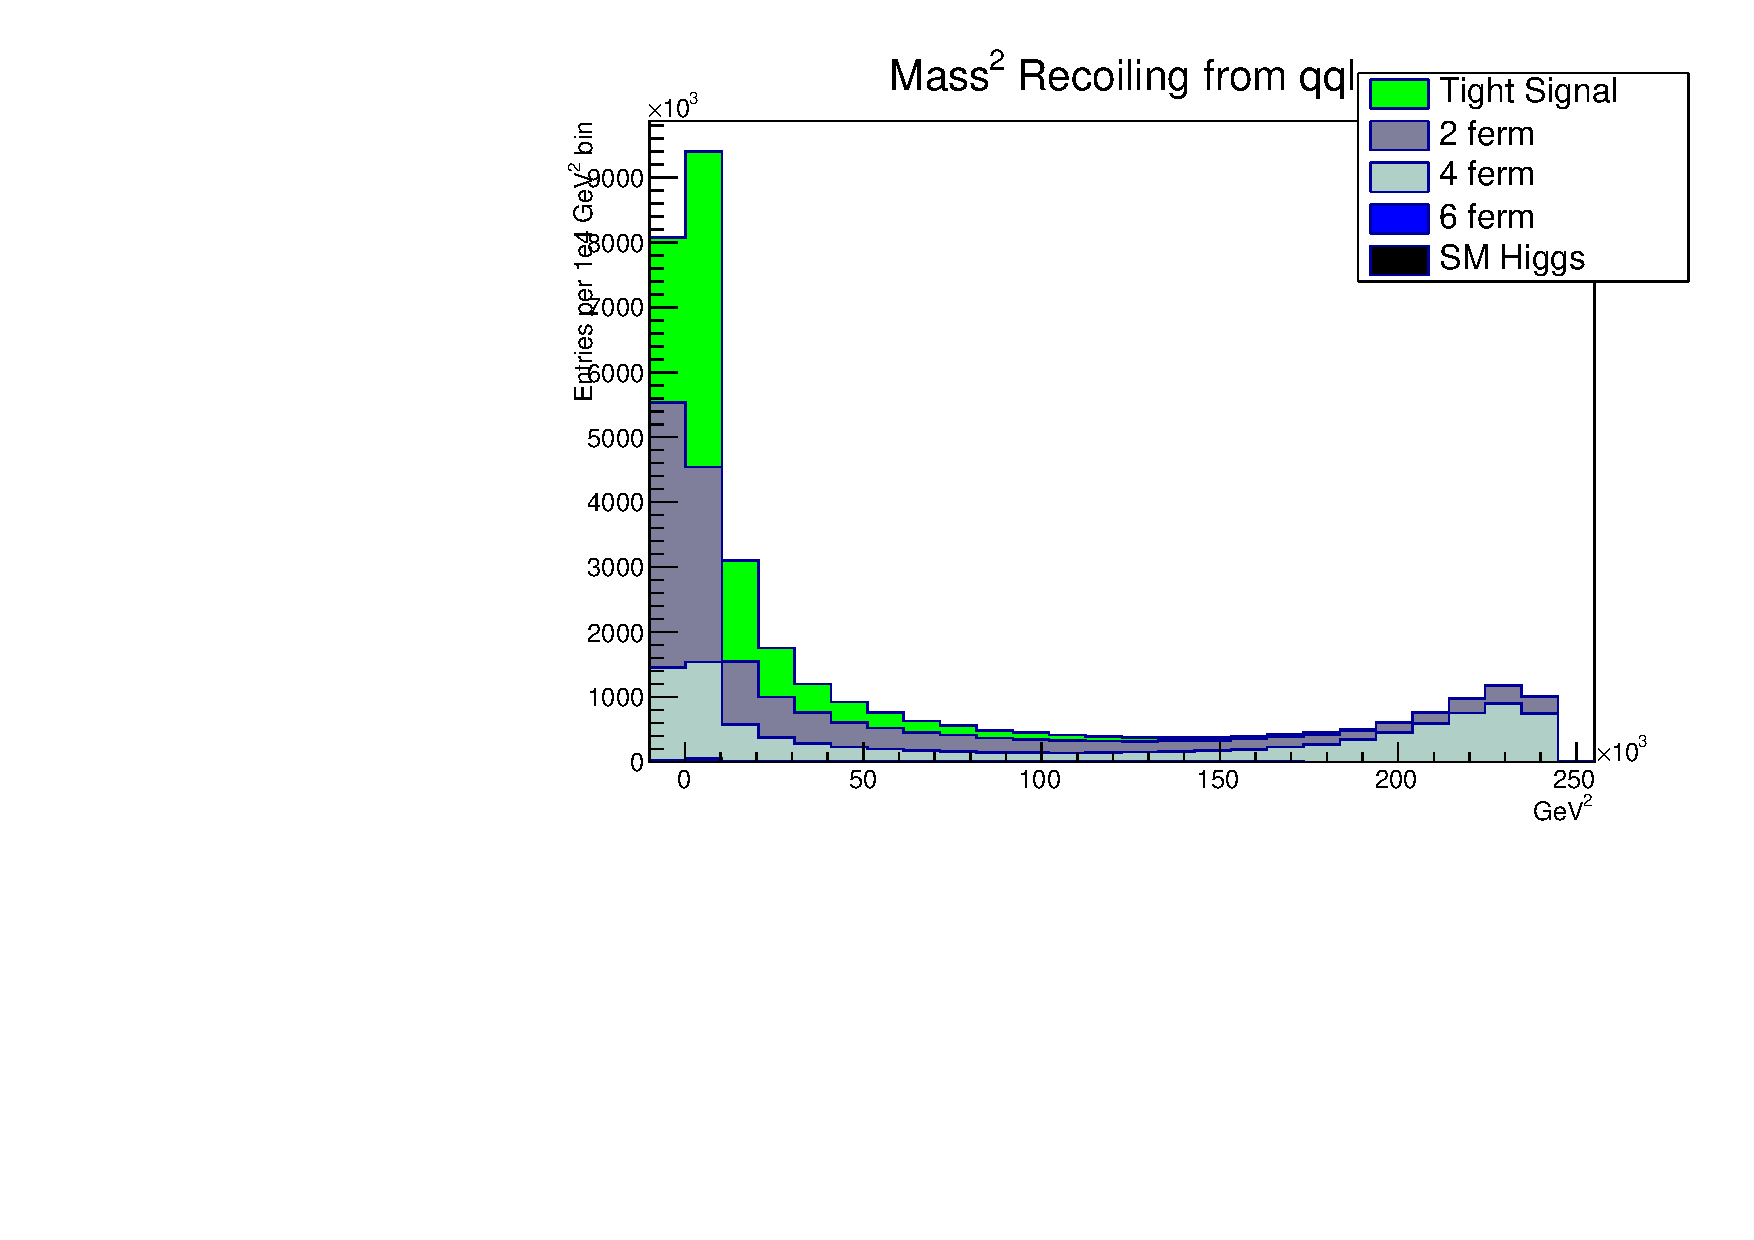
\includegraphics[scale=0.3, left]{vrecoilHist.pdf} \\
$m^2_{\nu recoil} < 135,000 \, \, \text{GeV}^2$
\end{column}
\end{columns}
\end{frame}
\begin{frame}{(3) Event Selection -- Example Distribution}
Tight Signal $\Rightarrow$  muon cone for $\mu,e,\tau$ signal events\\
Polarization: (-0.8,+0.3)\quad
Luminosity: 1600 fb$^{-1}$\\
Example: Hadronic mass distribution after all event selection cuts
\begin{center}
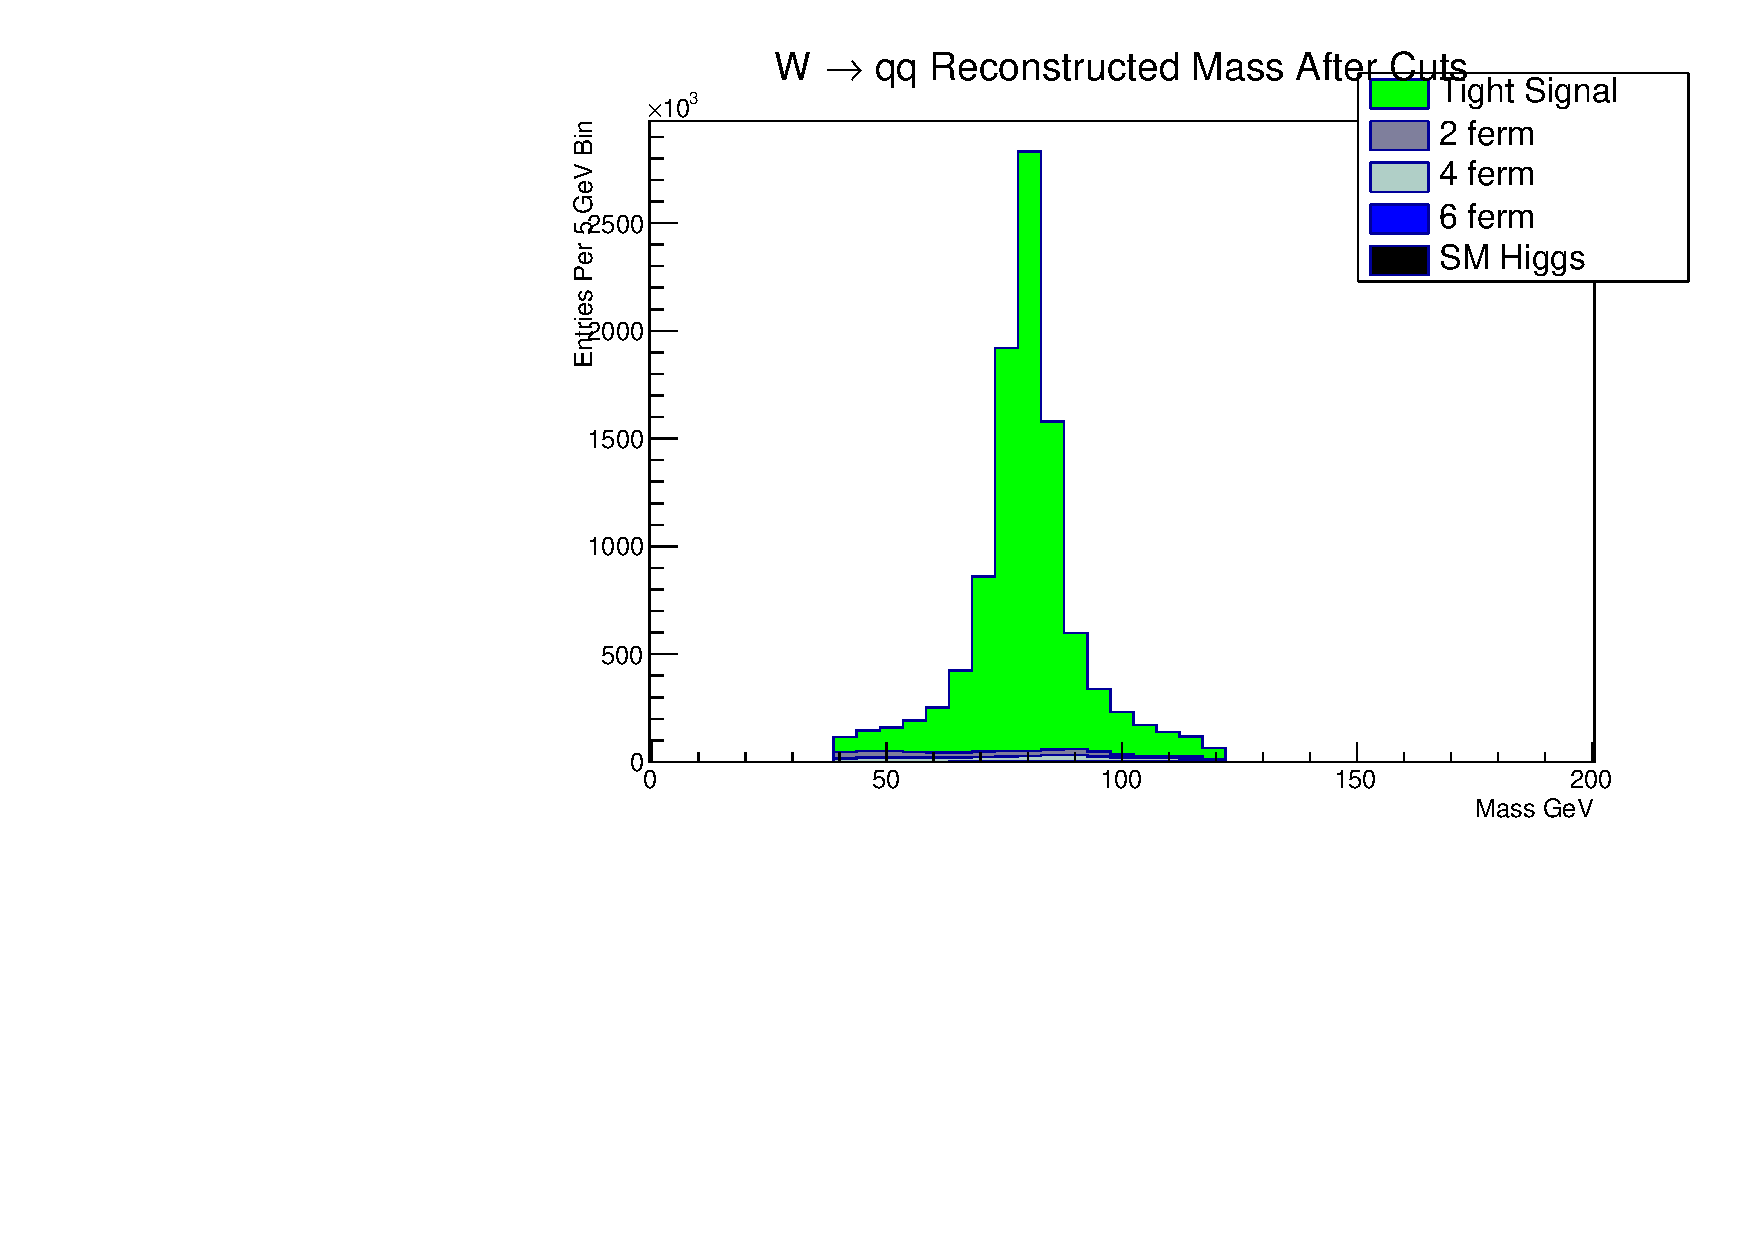
\includegraphics[scale=0.3, left]{mwhadCutsHist.pdf}
\end{center}



\end{frame}


\begin{frame}{(3) Event Selection -- ``WW-like" Signal}
\scriptsize
Polarization: (-0.8,+0.3)\quad
Luminosity: 1600 fb$^{-1}$
\makebox[\linewidth]{\parbox{12.5cm}{  %}}
\tiny
Tight Selection with muon cone\\
   \begin{tabular}{|p{0.09\textwidth}p{0.08\textwidth}p{0.08\textwidth}p{0.08\textwidth}p{0.08\textwidth}p{0.08\textwidth}p{0.08\textwidth}p{0.08\textwidth}p{0.08\textwidth}|}
\hline 
   & Prompt $\mu$ & Prompt $e$ & $\tau$ & Tot. Sig. & 2f & 4f & 6f & Higgs \\ \hline 
Base Evts &\num{3.87e+06 } & \num{3.89e+06 } & \num{3.90e+06} &\num{1.17e+07} & \num{4.22e+07} & \num{3.22e+07} & \num{2.14e+05} & \num{4.12e+05} \\ 

Lepton &\num{3.31e+06 } & \num{3.20e+06 } & \num{2.28e+06} &\num{8.78e+06} & \num{1.15e+07} & \num{1.18e+07} & \num{1.63e+05} & \num{1.15e+05} \\ 
 
$E_{vis}$ &\num{3.28e+06 } & \num{3.11e+06 } & \num{2.27e+06} &\num{8.67e+06} & \num{1.06e+07} & \num{1.15e+07} & \num{1.62e+05} & \num{1.11e+05} \\ 
 
N Tracks &\num{3.19e+06 } & \num{3.03e+06 } & \num{2.21e+06} &\num{8.43e+06} & \num{2.54e+06} & \num{2.59e+06} & \num{1.49e+05} & \num{8.89e+04} \\ 
 
$-qcos\theta$ &\num{3.18e+06 } & \num{3.01e+06 } & \num{2.18e+06} &\num{8.37e+06} & \num{2.19e+06} & \num{2.26e+06} & \num{1.44e+05} & \num{8.52e+04} \\ 
 
$M_{qq}$ $>$40 &\num{2.94e+06 } & \num{2.80e+06 } & \num{2.03e+06} &\num{7.77e+06} & \num{1.13e+06} & \num{1.33e+06} & \num{1.42e+05} & \num{7.56e+04} \\ 
 
$M_{qq}$ $<$120 &\num{2.72e+06 } & \num{2.57e+06 } & \num{1.83e+06} &\num{7.13e+06} & \num{5.68e+05} & \num{2.68e+05} & \num{2.02e+04} & \num{2.97e+04} \\ 
 
$E_{com}$ &\num{2.72e+06 } & \num{2.57e+06 } & \num{1.83e+06} &\num{7.13e+06} & \num{5.58e+05} & \num{2.65e+05} & \num{2.02e+04} & \num{2.96e+04} \\ 

Pt vis. &\num{2.69e+06 } & \num{2.55e+06 } & \num{1.81e+06} &\num{7.05e+06} & \num{3.21e+05} & \num{2.37e+05} & \num{2.01e+04} & \num{2.94e+04} \\ 

$m^2_{\nu recoil}$ &\num{2.69e+06 } & \num{2.54e+06 } & \num{1.80e+06} &\num{7.03e+06} & \num{2.93e+05} & \num{2.02e+05} & \num{1.94e+04} & \num{2.23e+04} \\ 
\hline 
\rowcolor{green}
 $\epsilon$ & $0.6944 \pm 0.0024$ & $0.6542 \pm 0.0023$ & $0.4616 \pm 0.0027$ &  $0.6032 \pm 0.0015$ & $0.006941 \pm 0.00012$ & $0.006255 \pm 7.6e-05$ & $0.09051 \pm 0.00023$ & $0.05407 \pm 0.00045$ \\ 
\hline
\end{tabular}
\quad \quad \\
Loose selection with tau cone\\
\begin{tabular}{|p{0.09\textwidth}p{0.08\textwidth}p{0.08\textwidth}p{0.08\textwidth}p{0.08\textwidth}p{0.08\textwidth}p{0.08\textwidth}p{0.08\textwidth}p{0.08\textwidth}|}
\hline 
   & Prompt $\mu$ & Prompt $e$ & $\tau$ & Tot. Sig. & 2f & 4f & 6f & Higgs \\ \hline 
Base Evts &\num{3.87e+06 } & \num{3.89e+06 } & \num{3.90e+06} &\num{1.17e+07} & \num{4.22e+07} & \num{3.22e+07} & \num{2.14e+05} & \num{4.12e+05} \\ 
 
Lepton &\num{3.36e+06 } & \num{3.30e+06 } & \num{2.82e+06} &\num{9.48e+06} & \num{1.30e+07} & \num{1.36e+07} & \num{1.77e+05} & \num{1.38e+05} \\ 

Tight Lep. Veto &\num{7.72e+04 } & \num{1.28e+05 } & \num{5.70e+05} &\num{7.76e+05} & \num{1.93e+06} & \num{2.15e+06} & \num{1.61e+04} & \num{3.12e+04} \\ 
 
$E_{vis}$ &\num{7.64e+04 } & \num{1.26e+05 } & \num{5.70e+05} &\num{7.72e+05} & \num{1.82e+06} & \num{1.94e+06} & \num{1.54e+04} & \num{3.02e+04} \\ 

N Tracks &\num{7.37e+04 } & \num{1.21e+05 } & \num{5.54e+05} &\num{7.49e+05} & \num{1.50e+06} & \num{1.64e+06} & \num{1.51e+04} & \num{2.71e+04} \\ 
 
$-qcos\theta$ &\num{6.30e+04 } & \num{1.12e+05 } & \num{5.32e+05} &\num{7.07e+05} & \num{1.11e+06} & \num{1.41e+06} & \num{1.45e+04} & \num{2.56e+04} \\ 
 
$M_{qq}$ $>$ 40 &\num{4.92e+04 } & \num{9.72e+04 } & \num{4.86e+05} &\num{6.33e+05} & \num{5.98e+05} & \num{1.30e+06} & \num{1.44e+04} & \num{2.33e+04} \\ 

$M_{qq}$ $<$ 120 &\num{4.04e+04 } & \num{7.81e+04 } & \num{4.16e+05} &\num{5.35e+05} & \num{2.58e+05} & \num{1.11e+05} & \num{1.11e+03} & \num{1.24e+04} \\ 
 
$E_{com}$ &\num{4.04e+04 } & \num{7.81e+04 } & \num{4.16e+05} &\num{5.34e+05} & \num{2.50e+05} & \num{1.10e+05} & \num{1.11e+03} & \num{1.24e+04} \\ 

Pt vis. &\num{4.00e+04 } & \num{7.74e+04 } & \num{4.12e+05} &\num{5.29e+05} & \num{1.17e+05} & \num{1.01e+05} & \num{1.11e+03} & \num{1.23e+04} \\ 
 
$m^2_{\nu recoil}$ &\num{3.94e+04 } & \num{7.70e+04 } & \num{4.07e+05} &\num{5.24e+05} & \num{1.02e+05} & \num{7.59e+04} & \num{1.02e+03} & \num{9.73e+03} \\ 
\hline 
\rowcolor{emerald}
 $\epsilon$ & $0.01017 \pm 0.00053$ & $0.01982 \pm 0.00071$ & $0.1046 \pm 0.0018$ &  $0.04495 \pm 0.00065$ & $0.002411 \pm 3.2e-05$ & $0.002356 \pm 3.7e-05$ & $0.004742 \pm 6.7e-05$ & $0.0236 \pm 0.00024$ \\ 


 \hline
 \end{tabular}

%end box
}}
\end{frame}
\begin{frame}{(3) Event Selection -- Not ``WW-like" Signal}
\scriptsize
Polarization: (-0.8,+0.3)\quad
Luminosity: 1600 fb$^{-1}$\\
Signal events containing off-shell W\\
 \scriptsize
Signal events with at least 1 off off shell(O.S.) W are separated into a new category of not ``WW-like" signal events
\tiny
\begin{columns}
\begin{column}{0.5\textwidth}
Tight Selection with muon cone\\
    \begin{tabular}{|p{0.18\textwidth}p{0.22\textwidth}p{0.21\textwidth}p{0.18\textwidth}|}
\hline 
 & Prompt $\mu$ O.S. & Prompt e O.S. & Tau O.S. \\ \hline 
Base Evts &\num{5.78e+05 } & \num{3.88e+06 } & \num{5.70e+05}\\ 

Lepton &\num{5.11e+05 } & \num{2.27e+06 } & \num{3.42e+05}\\ 
 
$E_{vis}$ &\num{5.08e+05 } & \num{2.25e+06 } & \num{3.41e+05}\\ 

N Tracks &\num{4.95e+05 } & \num{2.19e+06 } & \num{3.35e+05}\\ 
 
$-qcos\theta$ &\num{4.94e+05 } & \num{2.10e+06 } & \num{3.31e+05}\\ 
 
$M_{qq}$ $>$ 40 &\num{4.67e+05 } & \num{2.01e+06 } & \num{3.14e+05}\\ 

$M_{qq}$ $<$ 120 &\num{3.44e+05 } & \num{1.81e+06 } & \num{2.39e+05}\\ 
 
$E_{com}$ &\num{3.44e+05 } & \num{1.81e+06 } & \num{2.39e+05}\\ 

 Pt vis.&\num{3.40e+05 } & \num{1.80e+06 } & \num{2.36e+05}\\ 
 
$m^2_{\nu recoil}$ &\num{3.40e+05 } & \num{1.76e+06 } & \num{2.34e+05}\\ 
\hline 
\rowcolor{green}
 $\epsilon$ & $0.5882 \pm 0.006$ & $0.4535 \pm 0.0014$ & $0.4108 \pm 0.0063$ \\  \hline
\end{tabular}
\end{column}
\begin{column}{0.5\textwidth}
Loose Selection with tau cone\\
  \begin{tabular}{|p{0.18\textwidth}p{0.22\textwidth}p{0.21\textwidth}p{0.18\textwidth}|}
\hline 
   & Prompt $\mu$ O.S. & Prompt e O.S. & Tau O.S. \\ \hline 
Base Evts &\num{5.78e+05 } & \num{3.88e+06 } & \num{5.70e+05}\\ 

Lepton &\num{5.15e+05 } & \num{2.47e+06 } & \num{4.26e+05}\\ 
 
Tight Lep. Veto &\num{8.18e+03 } & \num{2.61e+05 } & \num{8.83e+04}\\ 
 
$E_{vis}$ &\num{7.87e+03 } & \num{2.61e+05 } & \num{8.83e+04}\\ 
 
N Tracks &\num{7.57e+03 } & \num{2.48e+05 } & \num{8.63e+04}\\ 
 
$-qcos\theta$ &\num{6.97e+03 } & \num{2.31e+05 } & \num{8.15e+04}\\ 
 
$M_{qq}$ $>$ 40 &\num{5.60e+03 } & \num{1.38e+05 } & \num{7.66e+04}\\ 
 
$M_{qq}$ $<$ 120 &\num{3.63e+03 } & \num{1.20e+05 } & \num{4.82e+04}\\ 
 
$E_{com}$ &\num{3.63e+03 } & \num{1.18e+05 } & \num{4.82e+04}\\ 

Pt vis. &\num{3.63e+03 } & \num{1.18e+05 } & \num{4.77e+04}\\ 
 
$m^2_{\nu recoil}$ &\num{3.63e+03 } & \num{9.15e+04 } & \num{4.73e+04}\\ 
\hline 

 $\epsilon$ & $0.006287 \pm 0.0011$ & $0.02358 \pm 0.00046$ & $0.08298 \pm 0.0038$ \\ \hline


\end{tabular} \\
\end{column}
\end{columns}
\scriptsize
-- selection is not that efficient for these types of events, and is not optimized to select these events
  

\end{frame}

\begin{frame}{Event Selection Summary (LR)}
 \tiny
 (-0.8, +0.3) 1600 fb${^-1}$\\
  \begin{tabular}{ |p{0.08\textwidth}|p{0.08\textwidth}p{0.08\textwidth}|p{0.08\textwidth}|p{0.08\textwidth}p{0.08\textwidth}p{0.08\textwidth}|} 
 \hline 
   &  \multicolumn{3}{|l|}{Tight Selection} &  \multicolumn{3}{|l|}{ Tight + Loose Sel.}  \\  \hline  
 & Sel. Total & Efficiency & Purity & Sel. Total & Efficiency & Purity \\ 
 \hline  
 Bkg. & 5.36e+05 & & & 7.25e+05 & &  \\ 
 Signal & 4.49e+06 & 0.578 $\pm$ 0.002 & 0.893  & 4.93e+06 & 0.635 $\pm$ 0.002 & 0.872 \\ 
 \rowcolor{orange}
 Sig.+O.S. & 6.93e+06 & 0.541 $\pm$ 0.001 & 0.928 & 7.47e+06 & 0.584 $\pm$ 0.001 & 0.912 \\ 
\hline 
\end{tabular} 
 \\
\normalsize
\quad \quad \\
\scriptsize
\begin{itemize}
\item[-] Signal is only on-shell WW-like events
\item[-] Signal + O.S.(Off-Shell) includes both selections including the not WW-like signal events
\item[-] in LR we find ratio of S/B to be 1 order of magnitude
\item[-] Good efficiency and high purity for the signal case
\item[-] When adding O.S. events we only strengthen the purity, but efficiency drops because the events are not ideal for selection
\end{itemize}
With Sig.+O.S. and Tight + Loose Sel.\\
\colorbox{yellow}{ $ \frac{\Delta\sigma}{\sigma} (stat.) = 0.04 \%$}
\end{frame}
\begin{frame}{(4) W-Mass Measurement }
Comparison of Generator mass differences\\
Polarization: (-0.8,+0.3)\quad
Luminosity: 1600 fb$^{-1}$\\
\scriptsize
\begin{columns}
\begin{column}{0.5\textwidth}
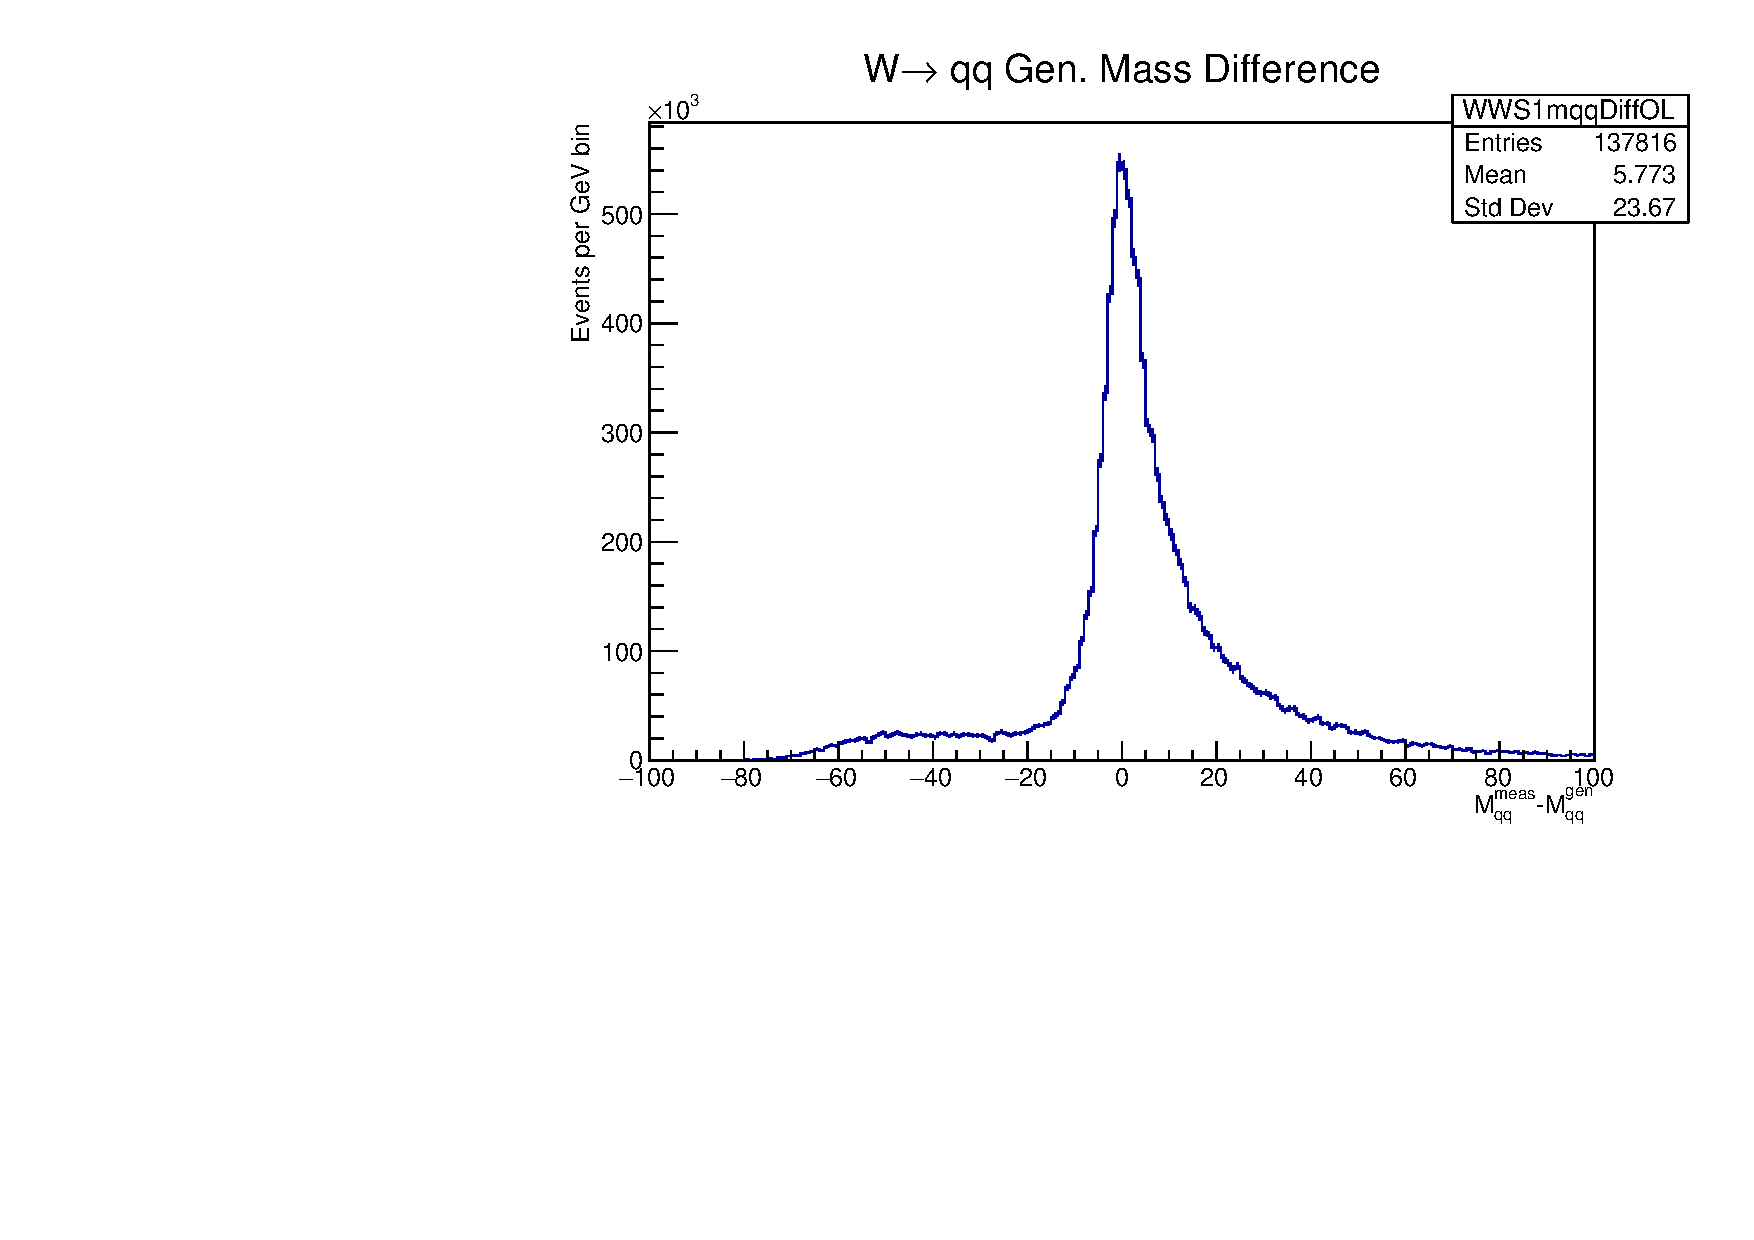
\includegraphics[scale=0.3, left]{mqqdiffOLHist.pdf} \\
Before Event Selection and pileup removal
\end{column}
\begin{column}{0.5\textwidth}

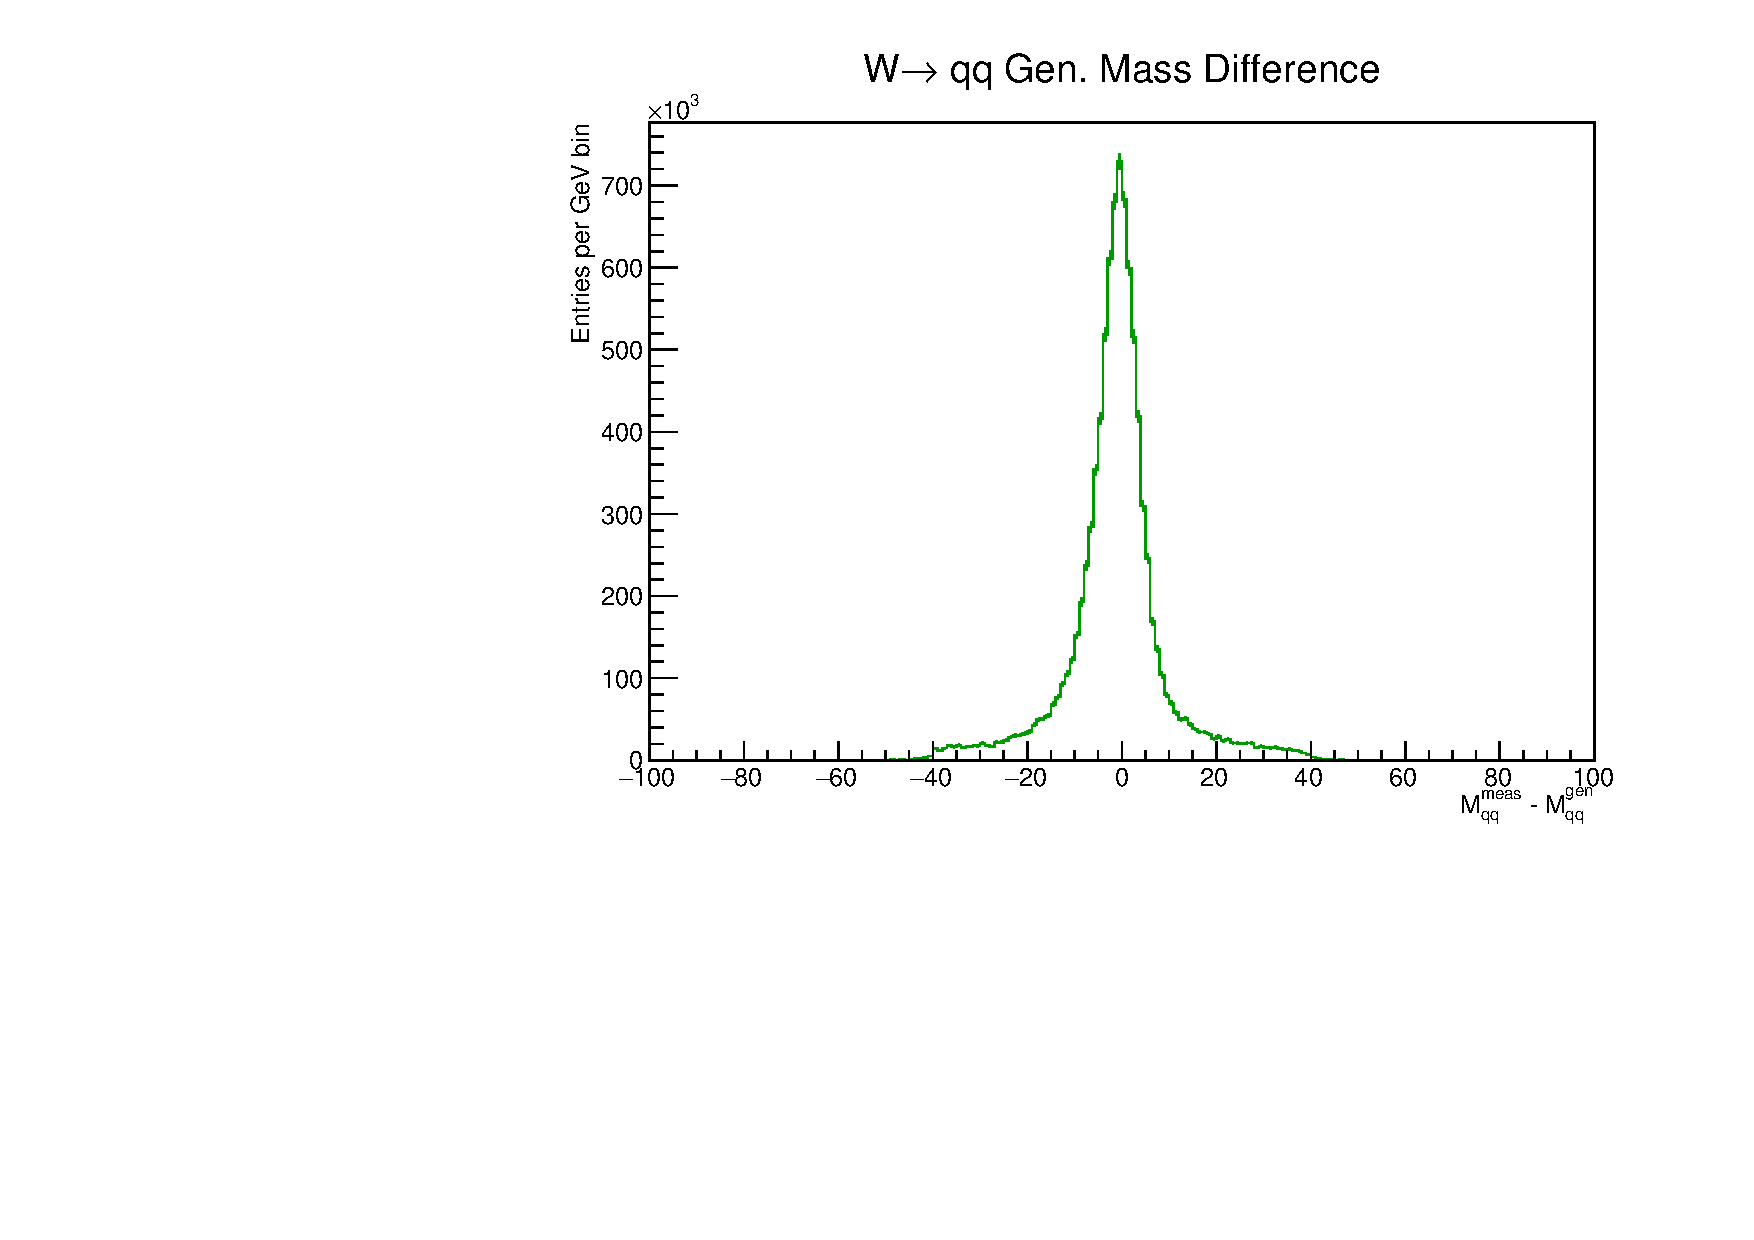
\includegraphics[scale=0.3, left]{mqqdiffHist.pdf} \\
After Event selection and pileup removal
\end{column}
\end{columns}
\quad \quad \\
\quad \quad \\


\end{frame}
\begin{frame}{(4) W-Mass Measurement }
Polarization: (-0.8,+0.3)\quad
Luminosity: 1600 fb$^{-1}$\\
Tight Signal+O.S. $\mu ,\tau$ only\\
\scriptsize
\begin{columns}
\begin{column}{0.5\textwidth}
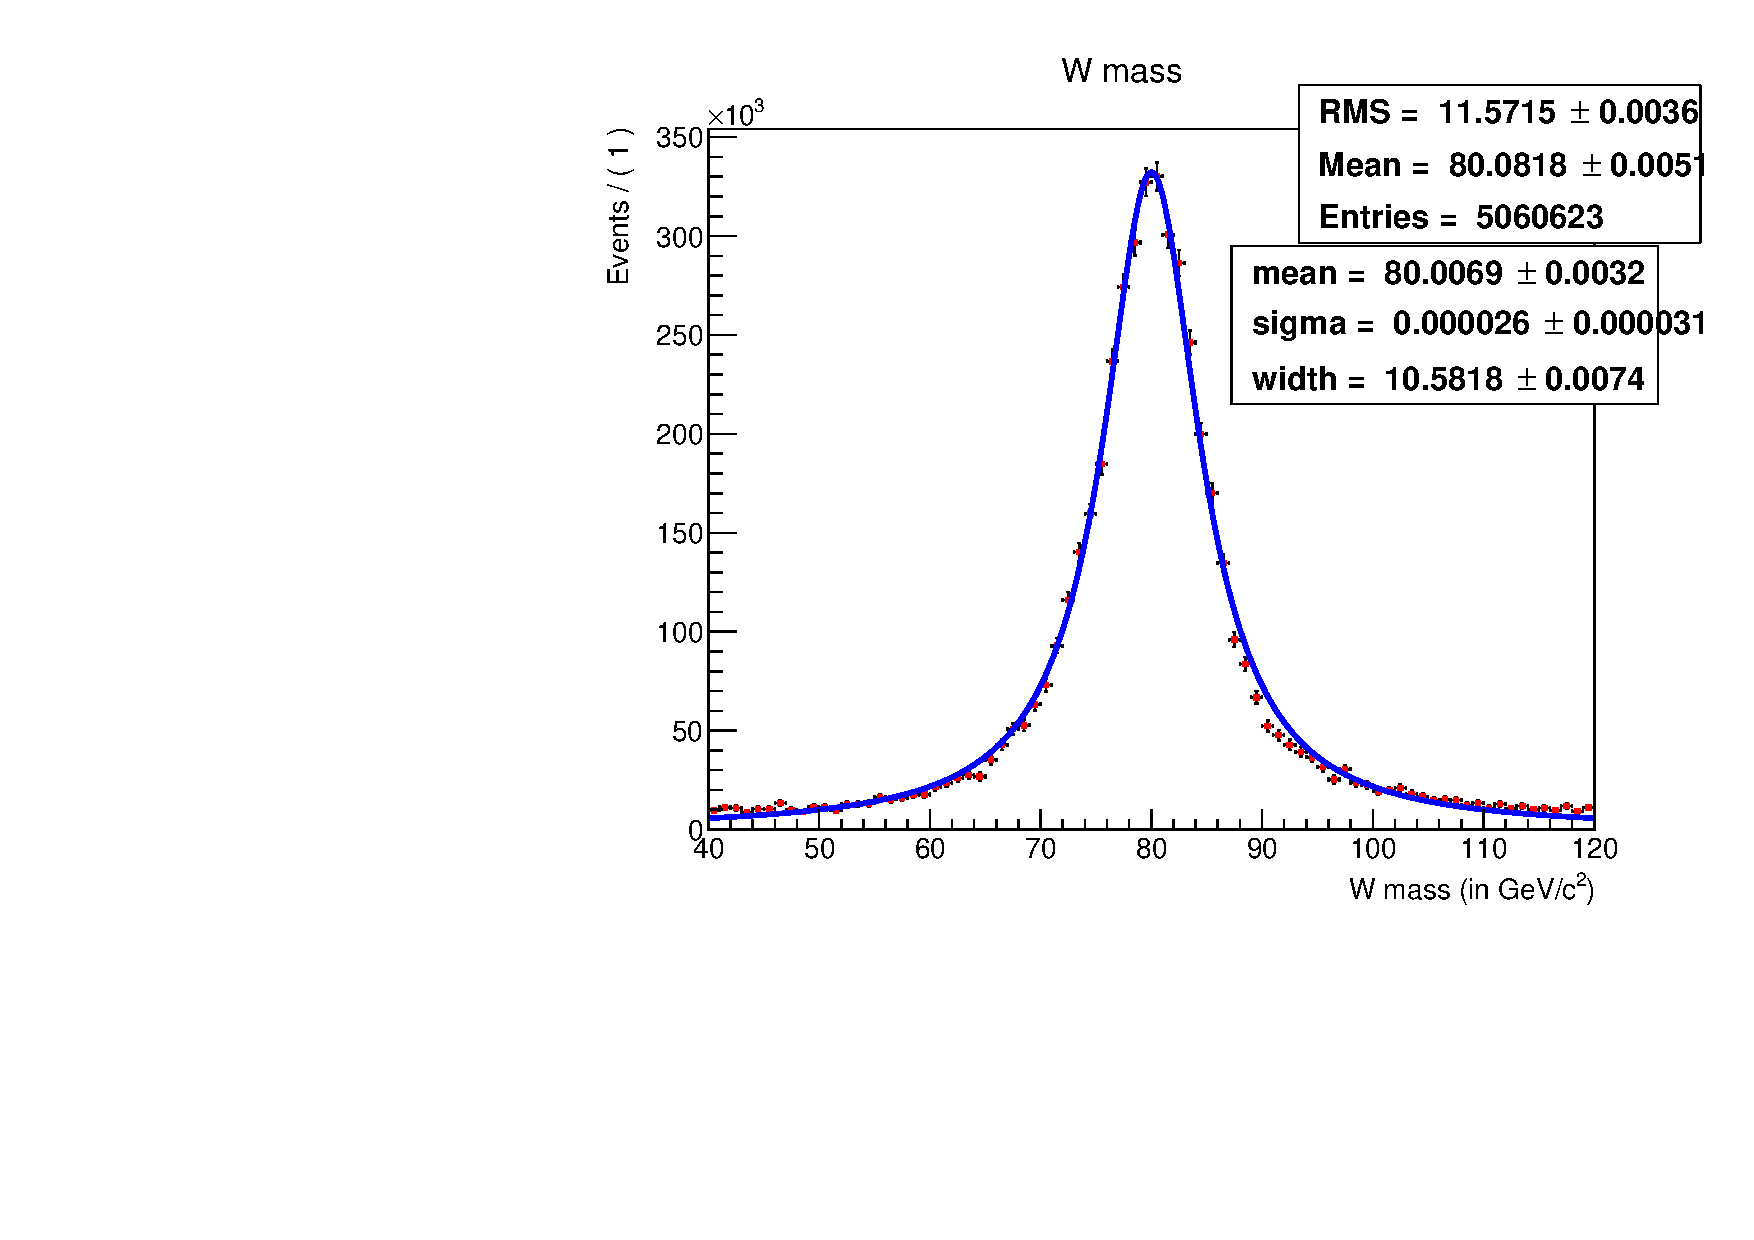
\includegraphics[scale=0.3, left]{WWSfit.pdf} \\
\begin{itemize}
\scriptsize
\item Applied Voigtian fit to get a model for W-mass shape
\item Poor fit, and statistical errors correspond to unweighted number of events
\end{itemize}
\end{column}
\begin{column}{0.5\textwidth}

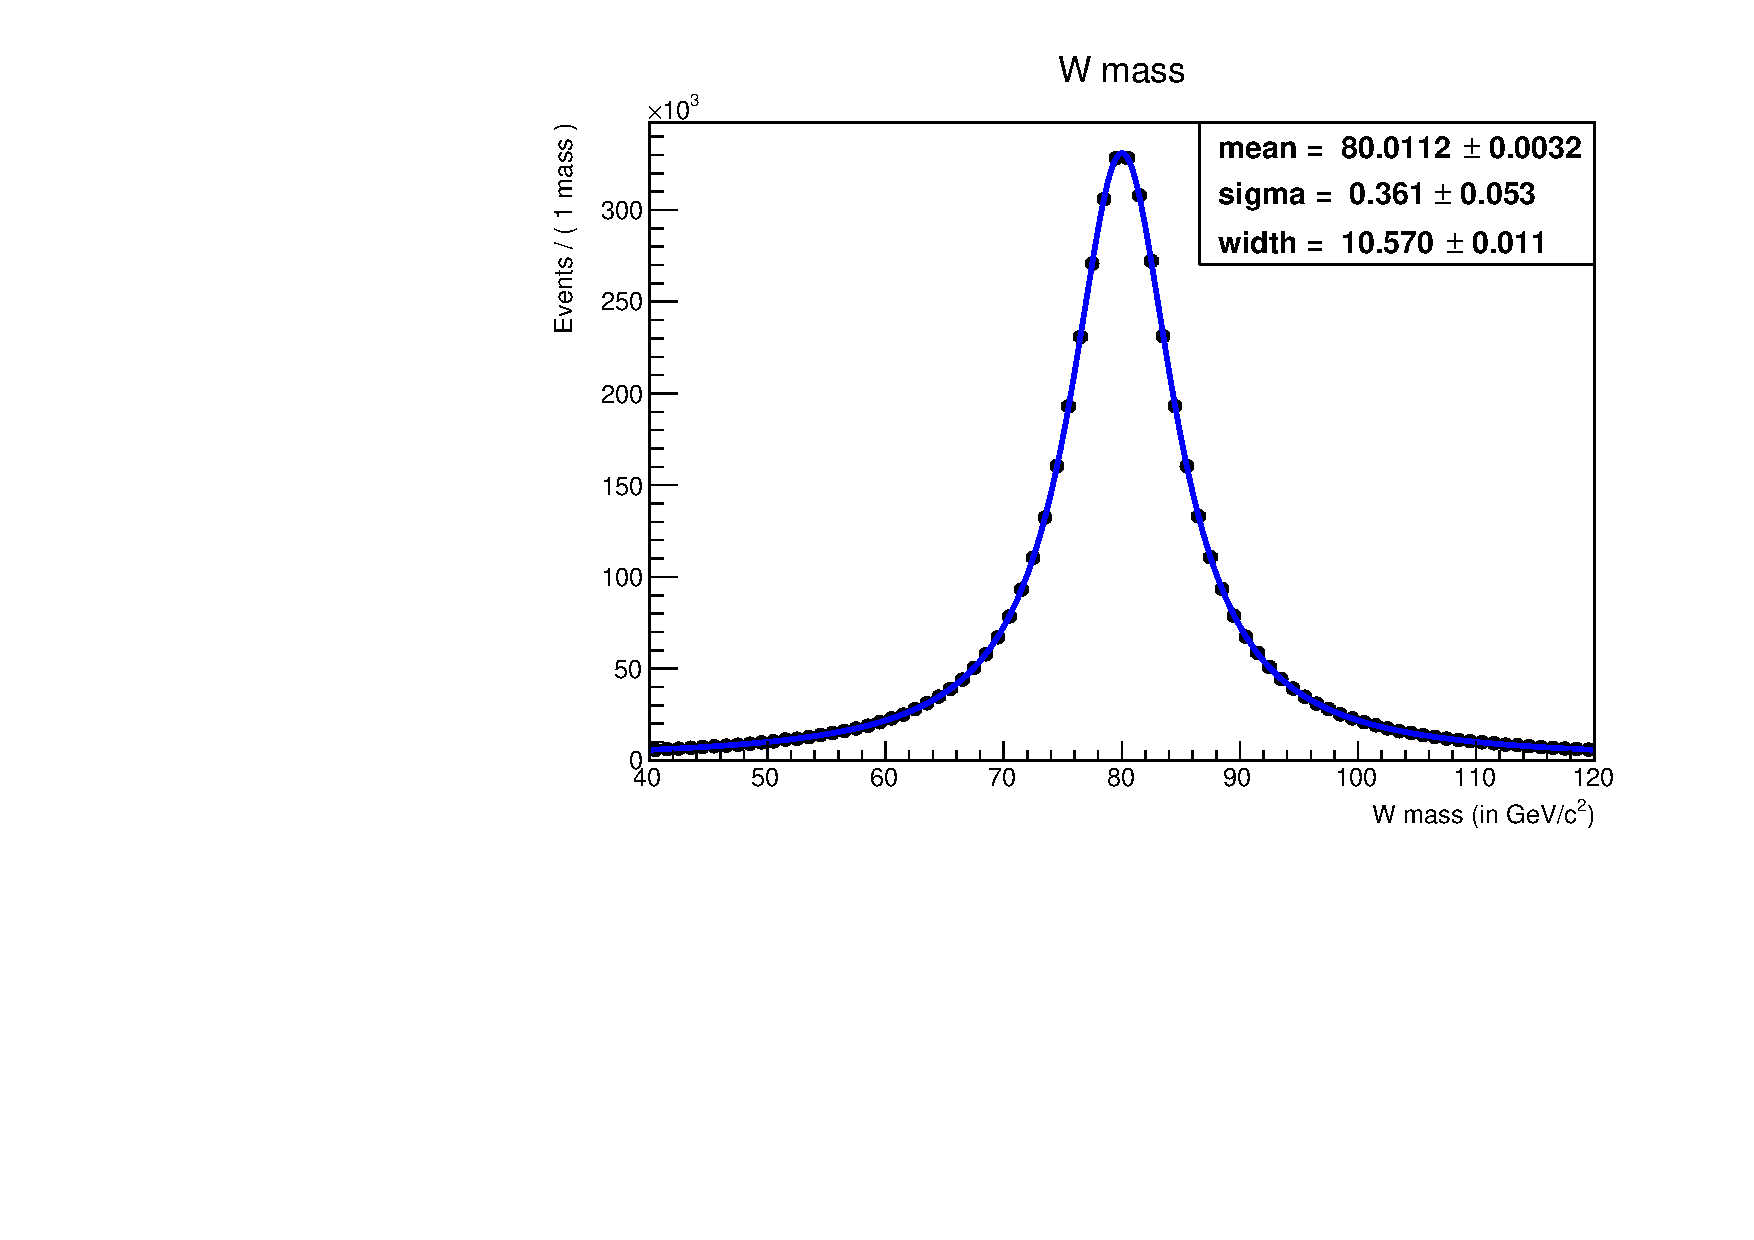
\includegraphics[scale=0.3, left]{toymass.pdf} \\
\begin{itemize}
\item Fit a toy model based on previous shape fit
\item Uses statistics consistent with 1600 fb$^{-1}$ (5.06M Events)
\item \colorbox{green}{$\Delta M_W (\text{stat.}) = 3.2 \, \text{MeV} \, \, \chi^2/ndof = 52.2/77$ }
\end{itemize}
\end{column}
\end{columns}
\quad \quad \\
\quad \quad \\

\end{frame}


\begin{frame}{Summary}
Completed Work:
\begin{itemize}
	\item[-] Performed a benchmarking analysis with $WW\rightarrow qq\ell\nu$
	\item[-] Treated the leptons universally with TauFinder
	\item[-] Rejected $\gamma \gamma$ pileup by fragmenting jets and making a Pt cut on the resulting mini-jets
	\item[-] Performed a basic event selection for all polarizations for a total of 4000 fb$^-1$ of data
	\item[-] Reported statistical errors $\Delta M_W$ and $\Delta\sigma$
	
\end{itemize}
TODO:
\begin{itemize}
	\item[-] Constrained fitting for W-mass and event selection improvements
	\item[-] Study efficiency as a function of $cos\theta$ of the lepton 
	\item[-] Separate muonic taus and prompt muons using IP significance or constrained fits

\end{itemize}

\end{frame}





\begin{frame}
Backup
\end{frame}
\begin{frame}{(1) TauFinder Optimization}
Optimization of 3 parameters:\\
-- searchCone $\in \, [0,0.15] $ rad with $0.01 $ rad steps\\
-- isolationCone $\in \, [0,0.15] $ rad with $0.01 $ rad steps\\
-- isolationEnergy $\in \, [0,5.5] $ GeV with $0.5 $ GeV steps \\

For simplicity, fix invariant mass cut at 3 GeV

Define optimization metrics:\\
\begin{columns}
\begin{column}{0.5\textwidth}
Efficiency using $WW\rightarrow qq l nu$ for
true leptons:\\
$\varepsilon_s = N_{matched}/N_{Stotal} $\\
	\scriptsize
	\quad -- a tau candidate is considered matched within 100 mrads of the gen lepton\\ 
	\quad -- if the gen lepton is a tau, the jet is matched to the gen visible components -- excluding FSR
	\quad -- $N_{Stotal}$ is the Number of events with 3 visible gen fermions $|cos\theta |< 0.99$
\end{column}
\begin{column}{0.5\textwidth}
fake leptons:
Use $WW \rightarrow qqqq$ \\
-- $\varepsilon_b = N_b/N_{Btotal}$ \\
	\scriptsize
	$N_b$ is any event with at least one reconstructed tau jet
\quad \quad \\

\quad 4 quarks give 4 chances to create a tau jet $\varepsilon_b$\\
--Use a better tuning parameter $P_{fake}$ which is the probability of reconstructing a tau jet from a single quark jet\\
\quad \quad \\
$P_{fake} = 1-(1 - \varepsilon_b)^{\frac{1}{4} }$\\
$\sigma_{P_{fake}} = \frac{1}{4} \sqrt{\frac{\varepsilon_b}{N_{Btotal} \sqrt{1-\varepsilon_b}} }$

\end{column}
\end{columns}

The optimal working point is chosen from the two tuning parameters max$[(1-P_{fake}) \varepsilon_s]$
\end{frame}

\begin{frame}{(3) Event Selection (Tight)}
Performance of hadronic mass and $W^{-}$ scattering angle\\
Polarization: (-0.8,+0.3)\quad
Luminosity: 1600 fb$^{-1}$\\
All cuts applied, tight selection only with $\mu ,e, \tau$

\begin{columns}
\begin{column}{0.5\textwidth}
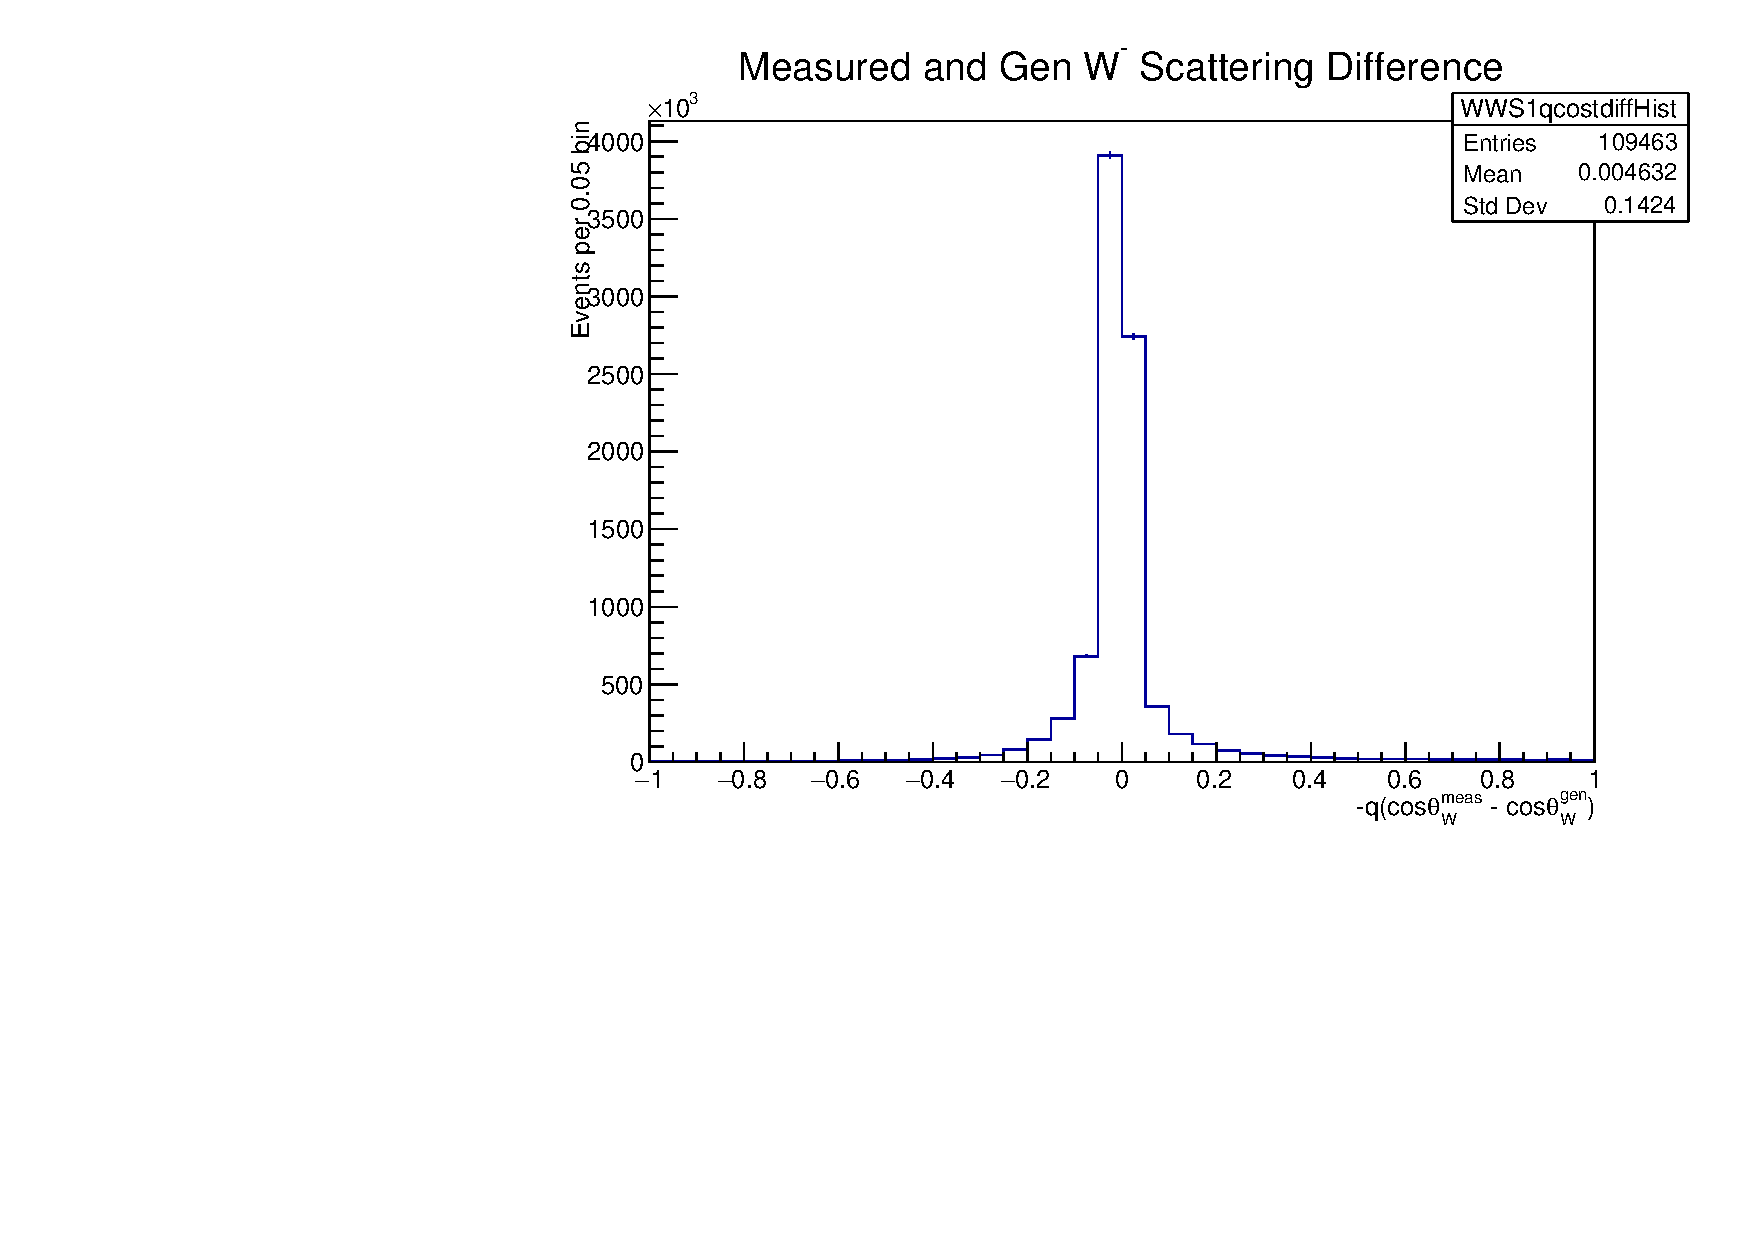
\includegraphics[scale=0.3, left]{qcostdiffHist.pdf} \\

\end{column}
\begin{column}{0.5\textwidth}
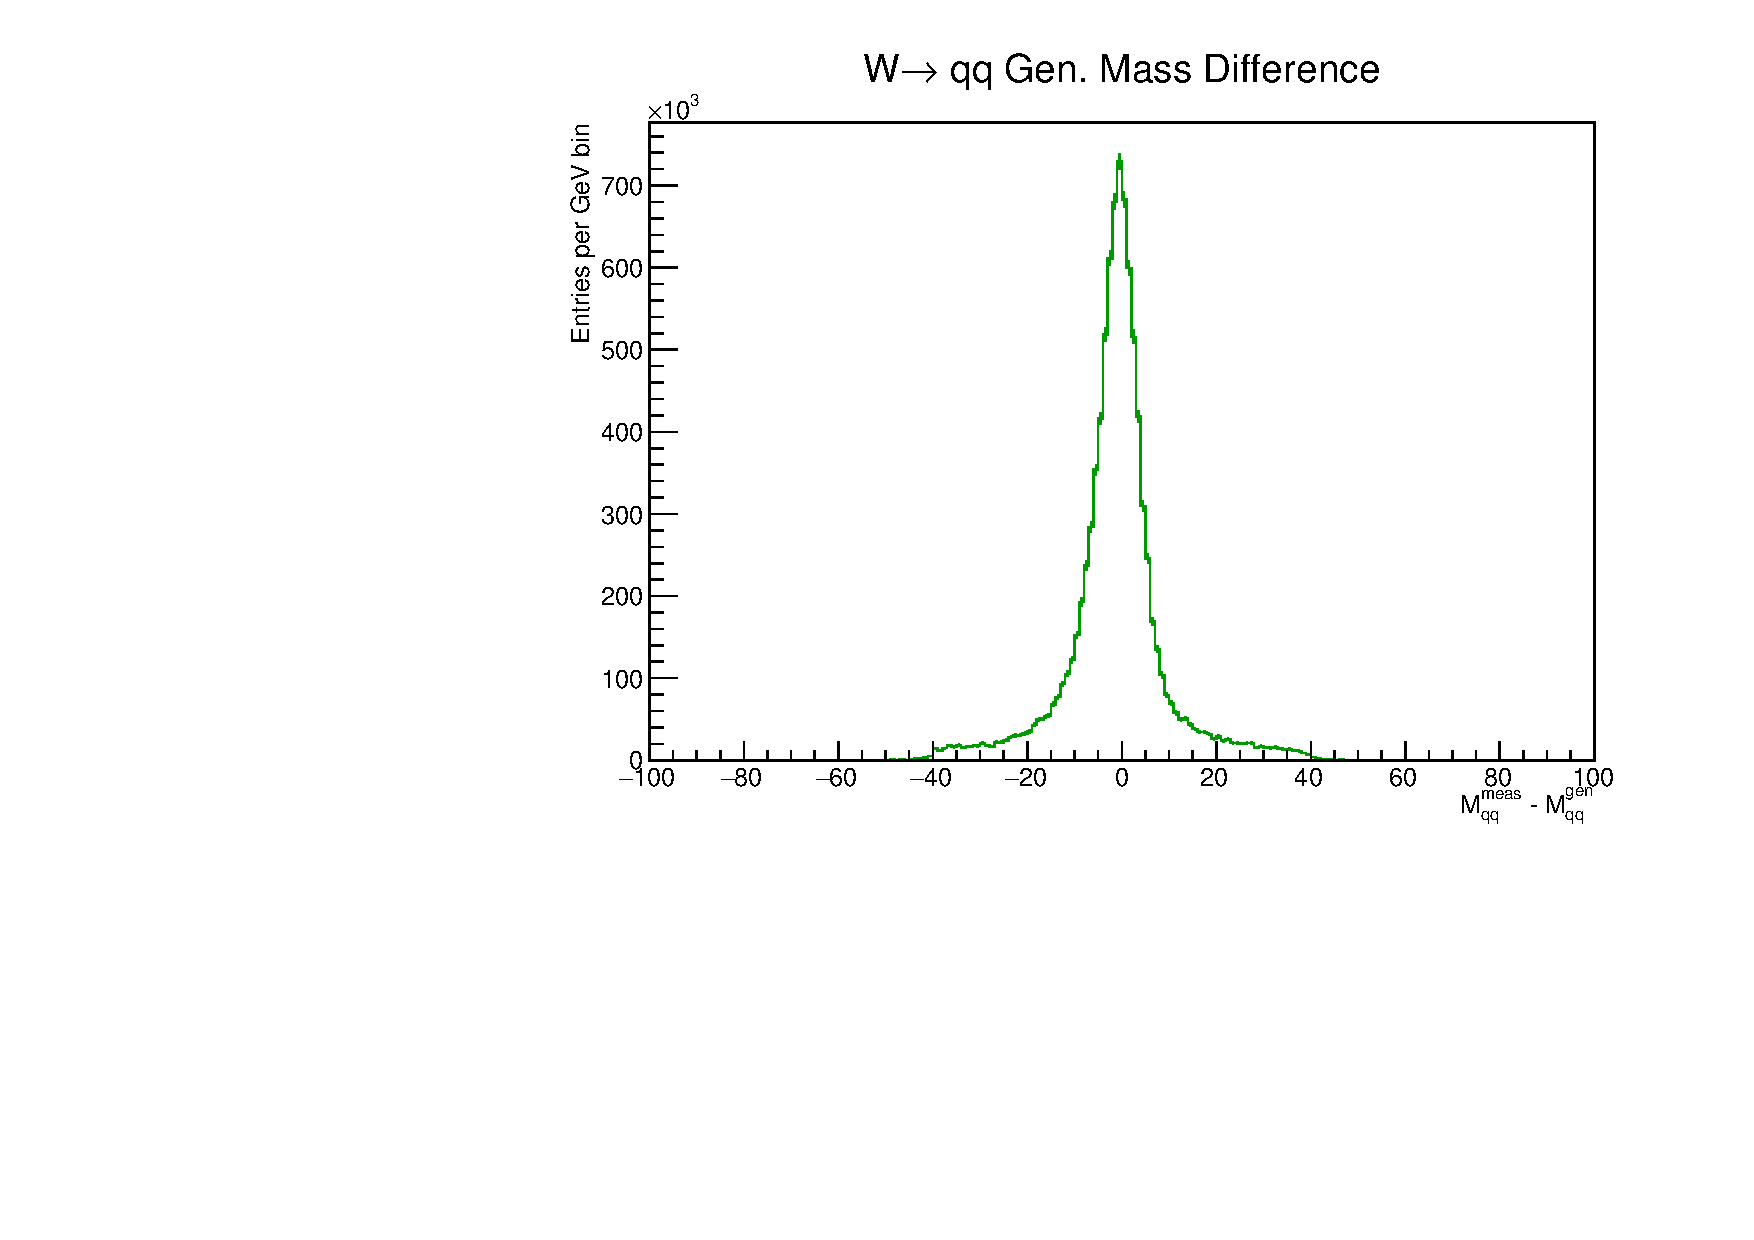
\includegraphics[scale=0.3, left]{mqqdiffHist.pdf} \\

\end{column}
\end{columns}

\end{frame}

\end{document}